	\documentclass[aps,superscriptaddress, notitlepage,longbibliography]{revtex4-1}

\usepackage{amsmath}
\usepackage{physics}
\usepackage[pdftex]{graphicx}
\usepackage{xcolor}
\usepackage{hyperref}
\setlength {\marginparwidth }{2cm}
\hypersetup{
    colorlinks,
    citecolor=blue,
    filecolor=black,
    linkcolor=red,
    urlcolor=blue
}

\newcommand{\comment}[1]{{\color{blue}#1}}
\newcommand{\edit}[1]{{\color{purple}#1}}
\newcommand{\del}[1]{{\color{red}\st{#1}}}
\newcommand{\beginsupplement}{%
        \setcounter{table}{0}
        \renewcommand{\thetable}{S\arabic{table}}%
        \setcounter{figure}{0}
        \renewcommand{\thefigure}{S\arabic{figure}}%
     }
% Standardize command font styles and environments
\newcommand{\doccmd}[1]{\texttt{\textbackslash#1}}% command name -- adds backslash automatically
\newcommand{\docopt}[1]{\ensuremath{\langle}\textrm{\textit{#1}}\ensuremath{\rangle}}% optional command argument
\newcommand{\docarg}[1]{\textrm{\textit{#1}}}% (required) command argument
\newcommand{\docenv}[1]{\textsf{#1}}% environment name
\newcommand{\docpkg}[1]{\texttt{#1}}% package name
\newcommand{\doccls}[1]{\texttt{#1}}% document class name
\newcommand{\docclsopt}[1]{\texttt{#1}}% document class option name
\newenvironment{docspec}{\begin{quote}\noindent}{\end{quote}}% command specification environment


\DeclareMathOperator*{\argmax}{arg\,max}
\DeclareMathOperator*{\argmin}{arg\,min}

\definecolor{pastel_green}{rgb}{0.18,0.65,0.34}
\newcommand{\CHW}[1]{\textcolor{pastel_green}{#1}}
%% OPTIONAL MACRO DEFINITIONS
\def\s{\sigma}


\def \M{\mathcal{M}}  
\def \P{\mathrm{P}}
\def \E{\mathbb{E}}


\def \mcl{\mathcal}
\def \mbb{\mathbb}
\def \mbf{\mathbf}



\def\bd{\boldsymbol}
\def\sm{\setminus}
\def\tb{\textbf}

\def\CH{\cal{H}} 

\def\<{\langle}
\def\>{\rangle}

\def\thet{{\theta}^{(t)}}
\def\thetp{{\theta}^{(t+1)}}
\def\thets{{\theta}^{(t)\star}}


\def\be{\begin{equation}} 
\def\ee{\end{equation}}
\newcommand \bea {\begin{eqnarray}} 
\newcommand \eea {\end{eqnarray}} 
\newcommand \sign {\hbox{sign}} 
\newcommand{\nn} {\nonumber}
\newcommand{\mbbE} {\mathbb{E}}
\begin{document}

\title{ scTOP: physics-inspired order parameters for cellular identification and visualization of developmental trajectories}

\author{Maria Yampolskaya}
\email{mariay@bu.edu}
\affiliation{Department of Physics, Boston University, Boston, MA 02215, USA}
\author{Michael Herriges}
\affiliation{Center for Regenerative Medicine of Boston University and Boston Medical Center, Boston, MA, USA}
\author{Laertis Ikonomou}
\affiliation{Department of Oral Biology. University at Buffalo, The State University of New York, Buffalo, NY, USA}
\affiliation{Division of Pulmonary, Critical Care and Sleep Medicine, Department of Medicine, University at Buffalo, The State University of New York, Buffalo, NY, USA}
\author{Darrell Kotton}
\affiliation{Center for Regenerative Medicine of Boston University and Boston Medical Center, Boston, MA, USA}
\affiliation{The Pulmonary Center and Department of Medicine, Boston University School of Medicine, Boston, MA, USA}
\author{Pankaj Mehta}
\email{pankajm@bu.edu}
\affiliation{Department of Physics, Boston University, Boston, MA 02215, USA}
\affiliation{Center for Regenerative Medicine of Boston University and Boston Medical Center, Boston, MA, USA}
\affiliation{Faculty of Computing and Data Science, Boston University, Boston, MA 02215, USA}
\affiliation{Biological Design Center, Boston University, Boston, MA 02215, USA}


\begin{abstract}
Recent advances in single-cell RNA-sequencing (scRNA-seq) and lineage tracing techniques provide an unprecedented window into the biology of cellular identity. The wealth of data calls for new theoretical and computational frameworks for understanding cell fate specification, accurately classifying cell fates from expression data, and integrating knowledge from cell atlases. Here, we present single-cell Type Order Parameters (scTOP): a statistical-physics-inspired approach for constructing “order parameters” for cell fate given a reference basis of cell types.  scTOP achieves near state-of-the-art performance for cell identification at the resolution of single cells and yields interpretable visualizations of developmental trajectories, such as bifurcations between closely related cell fates. Importantly, scTOP does this without using feature selection, statistical fitting, or dimensional reduction (e.g. UMAP, t-SNE, PCA, SPRING). We illustrate the power of scTOP on a wide variety of human and mouse datasets (both in vivo and in vitro), including existing tissue atlases and lineage tracing data. We also provide an easy-to-use Python package implementation of scTOP. Our results suggest that physics-inspired order parameters can serve as an important tool for understanding and analyzing developmental landscapes and cellular identity across biological contexts and organisms.
\end{abstract}

\maketitle

\section{Introduction}
Humans and other mammals have many specialized cells that arise through a complex developmental process  \cite{zeng_what_2022}. At early embryonic stages, cells are pluripotent and possess the flexibility to develop into fates from all three germ layers \cite{Wolpert_2019}. However, as embryos mature, cellular identity becomes less plastic and more specified through a complex spatiotemporal process involving signaling and environmental cues. The questions of how and why cells end up in one fate or another are fundamental to developmental biology [CITE]. More practically, understanding the process of cell fate specification is crucial for developing directed differentiation protocols for engineer cells \emph{in vitro}, with important clinical application for human health and disease [CITE].

One powerful set of techniques for characterizing cellular phenotype are transcriptome-wide measurements using single-cell RNA sequencing (scRNA-seq). Typical scRNA-seq experiments involve thousands of genes and dozens to millions of cells. For this reason, this data is intrinsically high-dimensional and requires specialized computational tools for analysis and interpretation [CITATION DUMP]. This task is especially difficult because the technical challenges of sequencing RNA from individual cells results in data that is noisy and sparse \cite{lahnemann_eleven_2020}. Genes with relatively low expression are often recorded as not being expressed at all, resulting in zero-counts called ``dropouts'' [CITE]. Experimental-to-experiment differences in sequencing method, platform, and other difficult-to-standardize conditions result in technical variations in scRNA-seq measurements called ``batch effects'' [CITE].These challenges merit careful consideration of how to normalize and analyze the data in a way that permits study of biological variation without conflation by technical variation.

scRNA-seq is often used for cellular identification. The most frequently used workflow involves applying dimensional reduction (such as UMAP \cite{mcinnes_umap_2018} or SPRING \cite{weinreb_spring_2018}) to visualize the data in two dimensions, then using unsupervised clustering to group individual cells. These groups are then often manually annotated according to expression levels of known marker genes [CITE]. Machine learning classifiers such as support vector machines are also commonly used identify cells after training with labeled data \cite{abdelaal_comparison_2019}. Another common analysis task is trajectory inference, where the goal is to infer developmental trajectories from static time shots [CITE]. Trajectory inference arranges cells on a low-dimensional manifold and assigns pseudo-times according to transcriptomic similarity. There are also methods like partition-based graph abstraction \cite{wolf_paga_2019} that purport to combine clustering and trajectory inference to simultaneously calculate pseudo-times and provide discrete labels at varying resolutions. 

Despite the power and utility of these computational tools, most commonly employed methods for scRNA-seq data share certain limitations. Dimensional reduction is often one of the first steps to analyze scRNA-seq data, but current methods highly distort cell-to-cell and cluster-to-cluster quantitative relationships \cite{chari_specious_2021}. Distorted embeddings inconsistently represent distances between individual data points and between cell types, making it difficult to interpret cell fate transitions. Similar issues arise in trajectory inference because  local neighborhoods can also vary substantially with the choice of embedding. Another limitation of these methods is the lack of reproducibility inherent to stochastic machine learning methods like t-SNE and UMAP, which output different results whenever they are executed  \cite{wattenberg_how_2016}. Many algorithms also perform feature selection (e.g., limiting there analysis to the most variable genes or highly-expressed genes) or require choosing parameters such as the perplexity, making results even more sensitive to the inclusion or exclusion of different datasets in the analysis [CITE].

An ideal analysis algorithm for scRNA-seq data should possess certain desirable properties. 
First, the algorithm should incorporate explicit assumptions that can be kept consistent between analyses. Second, the algorithm should be deterministic, further enhancing reproducibility. Third, the axes in visualization should be interpretable, intuitive, and remain fixed across analysis and datasets. Fourth, the algorithm should measure cell identity in a continuous way instead of assigning discrete identity labels, thus enabling a more subtle and fine-grained analysis of cellular identity and developmental trajectories. Finally, the algorithm should be easily able to incorporate datasets from multiple data sources, including the wealth of new single cell atlases now being generated [CITE].

Here, we present a new physics inspired algorithm, single-cell Type Order Parameters (scTOP), that has many of these properties. The algorithm is based on the statistical physics concept of an order parameter -- a coarse grained quantity that can distinguish between phases of matter. Arguably the most famous example of an order parameter is  magnetization in a ferromagnetic system (i.e., a system that can spontaneously magnetize). In a ferromagnet, the magnetization measures the alignment of spins and can be used to distinguish magnetic and paramagnetic phases [CITE STAT MECH]. It is straight forward to generalize the idea of magnetization to more complex settings such as spin glasses and attractor neural networks [CITE-AMIT]. In the context of epigenetic landscape models of cell identity, this takes the form of generalized magnetizations that measure how aligned a gene expression state is with each of the attractor basins for different cell fates \cite{lang_epigenetic_2014,pusuluri_cellular_2017}. These generalized magnetizations serve as natural order parameters for cellular identity and can be calculated directly from data \cite{lang_epigenetic_2014,pusuluri_cellular_2017, dame_thyroid_2017,ikonomou_vivo_2020}. The scTOP algorithm builds on previous work by developing methods for integrating scRNA-seq data, greatly expanding the power and utility of this approach. 
 
The inputs to scTOP are the scRNA-seq measurements of query data as well as a reference basis containing the archetypal gene expression profiles for cell types of interest. The output of scTOP are the coordinates  of the query data  in cell type order parameter space (i.e., generalized magnetizations), with each output dimension serving as a measure of similarity between the query data and a distinct cell type in the reference basis. In this way, scTOP naturally projects gene expression deterministically onto a space with dimension equal to the number of cell types in the reference basis. These generalized coordinates can be used for both cell type identification and visualization. One appealing feature of scTOP is that the assumptions of the algorithm are explicit and are contained entirely in the choice of reference basis. This allows direct comparison across datasets and settings since  the coordinates of, and distances between, data points do not change as long as one uses the same reference basis. One important limitation of scTOP worth noting  is that it cannot be easily used to identify novel cell fates. The underlying reason for this is that scTOP assumes one already know what cell types are of interest in the form of a reference basis and for this reason is poorly suited for exploratory work where the goal is to identify unknown cell types. 

In this paper, we show that scTOP can be used to reliably assess cell identity and accurately classify cell type with high accuracy at the resolution of individual cells.  We demonstrate this using mouse and human samples from lungs, brains, and other organs. By analyzing lineage tracing data and embryonic development data, we also establish scTOP's capacity to quantify transitions between cell types, including bifurcations between closely related cell fates.

We have implemented scTOP in an easy-to-use Python package, available on the Python Package Index [link] and Github [link], and an R package, available on Bioconductor [link] and Github [link]. All code, tutorials, and examples are available on the corresponding Github site [].

\section{Methods}
\begin{figure}
	\centering
		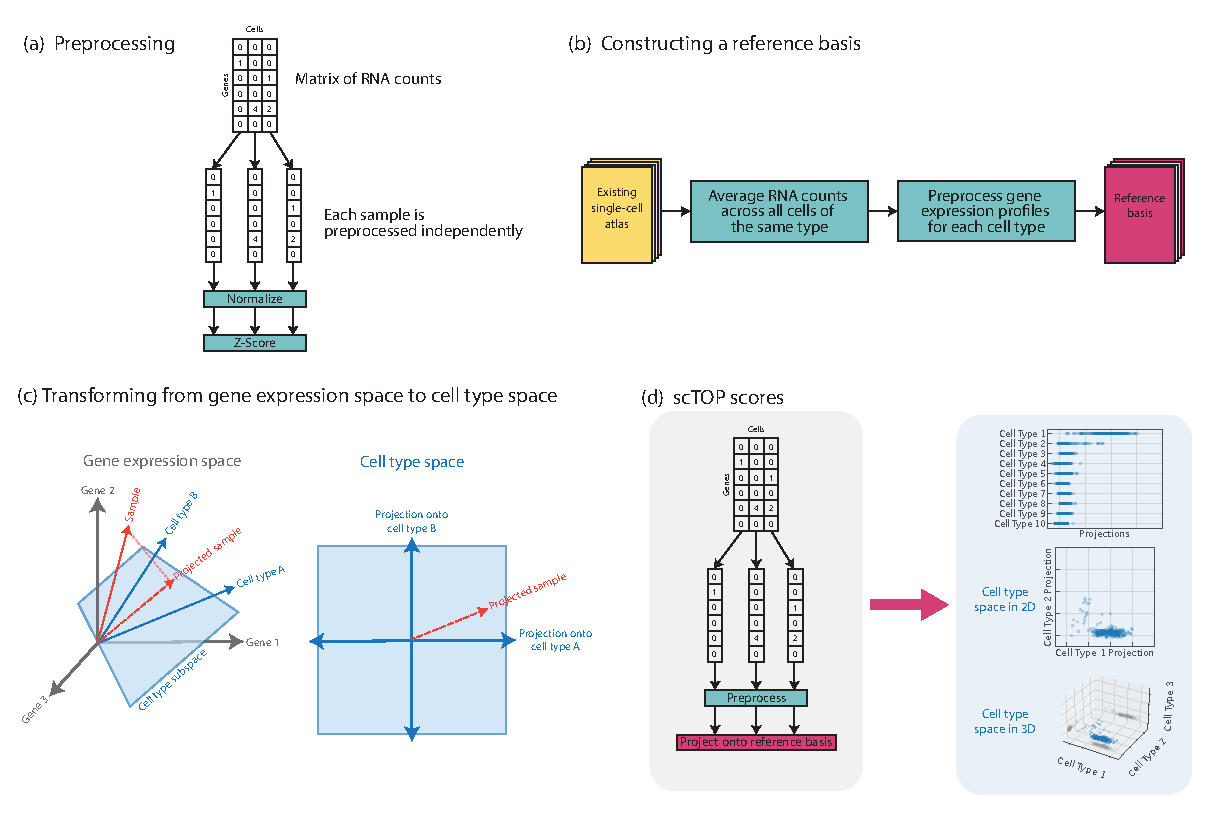
\includegraphics[scale=0.8]{figs/scTOP manuscript fig1 - no aggregate.pdf}
	\caption{Steps involved in the scTOP algorithm. (a) Each cell in the query data is pre-processed independently of the other cells in the dataset. (b) Single-cell RNA-seq atlases, such as the Mouse Cell Atlas, are used to define the reference basis in the algorithm. (c) scTOP scores are the projections of query data onto the non-orthogonal subspace of cell types. Since there is no statistical fitting, no tuning parameters are involved. (d) The process of finding scTOP scores is shown in the grey section, and the blue section illustrates cell-type space. This space has as many dimensions as there are cell types in the reference basis. We can visualize this concept in 1, 2, or 3 dimensions, depending on which cell types are most relevant. In the 3-dimensional case, the shadows on the bounds of the scatter plot are included to better illustrate the position of points in 3-dimensional space.}
	\label{FIG:1}
\end{figure}

To calculate cell type similarity scores, scTOP uses a linear algebra projection method inspired by the concept of cell types as attractors in a dynamical system \cite{huang_cell_2005}. This projection method has been applied previously to bulk RNA-seq samples, and we will summarize the theoretical background here \cite{lang_epigenetic_2014}. A cell type is a state of the gene regulatory network. A natural way to represent attractors in this system is with an attractor neural network, where attractors correspond to different cell types. If we represent each gene as a node in a network with an associated value measuring gene expression (positive value representing high gene expression, low value indicating low gene expression), then a cell type may be denoted by a vector of gene expression values $S_i$, where $i=1,\ldots, G$ spans the $G$ genes being measured.  The gene expression profiles
corresponding to the $C$ cell type attractors are also $G$ dimensional vectors $\xi_i^\mu$, where $\mu=1,\ldots, C$ spans the $C$ cell types being "stored" in the network. In what follows, we assume that $G > C$, namely the number of genes being measured is greater than the number of cell types.

Cell types are often highly similar in their patterns of gene regulation. Kanter and Sompolinsky \cite{kanter_associative_1987} defined a pattern storage method for spin-glass-like neural networks where even correlated patterns robustly act as attractors. For the same system, they also defined order parameters: generalized magnetizations $a^{\mu}$, where $\mu$ iterates through each of the stored cell type attractors. The $a^\mu$ can be understood as "decorrelated" versions of the conventional spin glass magnetization order parameter that measures the similarity between a given network state and the network state $\xi^\mu$. 
Explicitly, the $C$ generalized magnetizations $a^\mu$ can be calculated for a gene expression state $S_i$ via the expression
\be \label{op_eqn}
a^\mu= \sum_{\nu=1}^C\sum_{j=1}^G [A_{\mu \nu}]^{-1}\xi_j^\nu S_j.
\ee
where
\be
A_{\mu \nu}= \sum_{j}^G  \xi_j^\mu \xi_j^\nu,
\ee
is the overlap matrix of gene expression profiles of different cell types. As Lang et al. have shown, the order parameters $a^{\mu}$ provided an excellent similarity score for analyzing bulk RNA-seq data \cite{lang_epigenetic_2014}. However, bulk RNA-seq measurements average gene expression over many cells, rendering it impossible to measure cell fate transitions beyond an average tissue state. 

scTOP uses the same order parameters, $a^{\mu}$, to track cell type at the resolution of individual cells, making it possible to directly observe cells in different stages of differentiation. In both attractor neural networks and previous applications to bulk RNA-seq data, the expression vectors $S_i$ were binary variables. However, we have found that for working with scRNA-seq data it is helpful to treat $S_i$ as continuous. 

The first stage of the algorithm is preprocessing and normalization of the the input data. Importantly, in our algorithm measurements from each cell are normalized independently and do not depend on the expression profiles of any other cells in the dataset. In the raw scRNA-seq data for each cell, each gene has an integer value which counts the number of corresponding RNA reads. Genes are then rank-ordered. The rank order is then converted to a z-score assuming a normal distribution, representing the percentile rank of the expression of a gene within the cell relative to all other genes being measured. For example, a gene that has higher expression than $97.8\%$ of genes being measured is assigned a score of $z=2$, while a gene that has higher expression than half of genes is assigned a score of $z=0$. The details of the process and its effects on data distributions are described in Appendix section \ref{preprocessing}.

The structure of pre-processing before applying the projection method is a vital component of the algorithm, as shown in figure \ref{FIG:1} (a). Each cell is pre-processed independently, unlike other algorithms which process data across samples to find, for example, the most variable genes. By processing each cell independently, the output for one cell is independent of which other cells are being analyzed. Although the strength of scTOP is in its ability to analyze single cells, it's also possible to analyze gene expression levels averaged across cell populations. This can be useful in cases where one wants to probe selected subsets of cells at low resolution; for example, if one wants to identify pre-defined clusters of cells.

scTOP involves one-shot learning, and there is no stochasticity involved; the algorithm will produce the same output regardless of the particular instance of execution. There are no hyper-parameters involved in the training, which bypasses another source of bias. The only assumptions involved in the algorithm are explicit: that the gene expression profiles included in the reference basis are truly representative of the relevant cell types, and that the cell types included are indeed distinct cell phenotypes. 

Constructing a representative, accurate reference basis that is relevant to the data being analyzed is vital to the scTOP algorithm. This process is shown in figure \ref{FIG:1} (b). First, relevant single-cell RNA-seq atlases are gathered to be processed. For example, in analyzing mouse lung cells, we used the Mouse Cell Atlas \cite{noauthor_mapping_nodate}, which contains single-cell samples of mouse tissues across all major organs. Once the relevant atlases are identified, we take an average across each cell population that corresponds to a distinct cell type. It is important that enough cells are included in each average, in order to mitigate the potent effects of noise. The minimum sample size to achieve reasonable results is 200 cells. Noise affects the algorithm most strongly when it appears in the basis, since the de-correlation operation involved in the projection separates cells according to the canonical expression levels included in the reference basis. After each cell population is averaged to create the gene expression profiles for the desired cell types, each cell type profile is pre-processed separately using the same procedure as that used for processing single cells: normalization followed by z-scoring . This creates a modular reference basis where cell types can easily be replaced, removed, or added at will. 

Although they were originally inspired by attractor neural networks and spin glass physics, the order parameters $a^{\mu}$ can also be understood as non-orthogonal projections onto the subspace of cell type space. This idea is shown in figure \ref{FIG:1} (c). A single-cell RNA-seq measurement of a sample produces a list of values corresponding to the expression levels of different genes, and thus can be conceptualized as a vector in $G$-dimensional gene expression space, where $G$ is the number of genes. Single-cell RNA-seq atlases provide reference gene expression profiles for hundreds of known cell types; these reference profiles also exist as vectors in gene expression space. If we compile a reference basis consisting of reference profiles corresponding to cell types, these vectors span a $C$-dimensional subspace of gene expression space, where $C$ is the number of cell types in the basis. There are far more genes than cell types: $C < G$. We can project the measured sample vector onto the cell type subspace in order to find the coordinates in cell type space, which enables identification of individual cells and tissues. Since the cell type profiles are largely correlated, they form a non-orthogonal subspace, and the projection onto this space is a non-orthogonal projection.

We can write the sample vector as a sum of the projected components and the component perpendicular to the cell type subspace: 
\be
S_i = \sum_\mu a^{\mu} \xi^{\mu}_i + S^{\perp}_i,
\ee
where $S^{\perp}_i$ is the expression level of the $i$th gene of the component of the sample vector that is perpendicular to the cell type subspace. $S^{\perp}$ is the part of the sample vector that is not explained by the known cell types. It results from biological processes such as cell cycle variation and non-biological sources such as scRNA-seq noise. 

There are two types of scTOP scores: aggregate and individual. The aggregate scoring method is useful for analyzing identified sub-populations of data at once. The scores tend to be higher, since aggregating gene expression data decreases the effects of noise. In aggregate scoring, the raw RNA count data is averaged across each sub-population, and then these average gene expression profiles are pre-processed and projected onto the reference basis. See figure \ref{FIG:1} (d). The resulting scTOP score provides the location of the sub-population in the cell type dimensions specified by the reference basis, which can be visualized in one, two, or three dimensions by selecting one, two, or three relevant cell types. In individual scoring, as shown in figure \ref{FIG:1} (e), each individual cell is pre-processed and projected onto the reference basis separately. Due to the well-documented effects of scRNA-seq noise [CITE], the resulting scores tend to be lower. Nonetheless, the resulting scores are able to accurately and reproducibly identify and track individual cells through cell type space, in whatever number of dimensions (i.e. cell types) one chooses.

The crux of scTOP is choosing a good reference basis. scTOP scores are reliable when the input reference basis incorporates many cells and represents a wide, relevant set of specialized cell types. Since scRNA-seq data is noisy and dropout is prevalent, many cells of each reference cell type must be included in order to create representative gene expression profiles. The choice of cell types in the basis is vital, too. The main underlying assumption of scTOP is that the reference cell types accurately represent attractors of the gene regulatory network. If the cell types aren't sufficiently different from one another, as in early embryonic development or certain stromal cells where the same cell type is compared between organs, the resulting scTOP scores may be unreliable; exhibiting extreme sensitivity to small changes in the basis or becoming incoherent. More information on the limitations of scTOP may be found in appendix [insert appendix num.]. Generally, outside these very limited edge cases, we have found that scTOP can reliably distinguish even extremely closely related cells such (see example of pulmonary alveolar type 1 and type 2 cell lineages below).

The accuracy of cell type information that scTOP can extract from scRNA-seq is limited by the low signal-to-noise ratio. As shown in appendix [insert appendix num.], the scTOP scores for false identities form a Gaussian distribution around zero. These distributions give an estimate of error. In aggregate scTOP scoring, RNA counts are averaged across a population and the resulting score is generally higher for relevant cell types than the average individual scTOP score for the same population. This is because the averaging step in aggregate scoring mitigates the effects of sparsity and noise in the RNA count matrices due to dropout.

Many other methods for classifying and tracking cell type can be computationally intensive. Dimensional reduction methods like t-SNE involve finding the distance between every pair of points in the data set. For scRNA-seq data with $G$ genes and $N$ cells, this involves computing the $G$-dimensional distance between every pair of $N$ cells. While there are optimized ways to calculate this, it can be time-consuming when you are working with thousands to millions of cells. The core of the scTOP is equation \ref{op_eqn}, which only involves matrix inversion and multiplication. The matrix inversion only involves the reference basis (which contains $C$ cell types), so it only needs to be computed once. When applying scTOP to $N$ cells, the computation that scales with the number of cells is the multiplication of a $C \cross G$ matrix with a $G \cross N$ matrix. Modern programming libraries like Numpy are highly optimized for simple linear algebra functions; the result is that scTOP takes milliseconds to run, even for very large datasets. While other methods involve time- and memory-intensive statistical fitting, scTOP is fast b.

\section{Results}

\subsection{Benchmarking and validation: Classification of cell fate}
{\color{red}: This section is already pretty good -- I think just a little terse -- we have to talk up all the results a little bit by comparing to existing methods putting things in context -- 2-3 sentences at end of each example -- remember people think exactly what you tell them -- so tell them/show them why each example is impressive}


scTOP scores reliably and accurately identify the cell types of individual cells as well as of clusters of cells. To show this, we applied the algorithm to several scRNA-seq datasets across species and across laboratories. scTOP is organism-agnostic as long as an appropriate reference basis is used. Mice and humans are among the most common subjects of scRNA-seq measurements. Many atlases across organs and stages of development have been created for both species. We used some of these atlases, such as the Mouse Cell Atlas \cite{noauthor_mapping_nodate} and the Atlas of Lung Development \cite{negretti_single-cell_2021}, as reference bases to analyze datasets from various sources.

Table \ref{table:1} lists each of the datasets examined in this paper with their respective scTOP score accuracies. ``TopN" refers to the percent of cells whose true cell types were in the top ``N" scTOP scores, with a score greater than 0.1. "Unspecified" refers to the percent of cells for which the highest scTOP score was less than 0.1; this represents a failure of the algorithm to confidently identify the cell. The accuracies across species and tissues are high and the unspecified percentages are very low, even in dataset exceeding a million cells.

\begin{table}[h!]
\centering
\begin{tabular}{| c | c | c | c | c | c | c |}
\hline
Query Data & Species & Reference Basis & Top1 (percent) & Top3 (percent) & Unspecified (percent) & Total cells \\ 
\hline
Kotton lab & Mouse & Mouse Cell Atlas & 97.19 & 99.77 & 2.69 & 4,805 \\ 
\hline
Brain atlas & Mouse & Self & 86.28 & 96.89 & 1.78 & 1,161,041 \\
\hline
CellBench & Human & Self & 100 & 100 & 0 & 2,822 \\
\hline
Lung atlas & Human & Self & 79.78 & 85.16 & 3.32 & 2,952 \\  
\hline
\hline
Data set & Species & Reference Basis & Top1 (percent) & Top3 (percent) & Unspecified (percent) & Number of cell types \\
\hline
Mouse Cell Atlas & Mouse & Tabula Muris & 79.17 & 87.5 & 0 & 48 \\
\hline

\end{tabular}
\caption{Accuracy scores of included sample types for each the described data sets.}
\label{table:1}
\end{table}
{\color{red}: PM: We should say how well we do compare to other methods here-- does not have to be comprehensive but should show we perform about as well as SOTA --few sentences and revisit below each example -- beat this horse until it's dead.}



\subsubsection{Example 1: Lung lineages}
To demonstrate the efficacy of scTOP in the case where the reference basis and query data come from different sources, we projected mouse lung data from Herriges et al. \cite{herriges_durable_2022} onto the mouse cell atlas. The Herriges et al. dataset  measures gene expression levels of six different specialized lung types from mice used as control samples. See figure \ref{herriges} (a). The reference basis used to find the individual scTOP scores for this data set was derived from the Mouse Cell Atlas. Despite the fact that the Herriges et al. dataset and the Mouse Cell Atlas were created in different laboratories and different sequencing methods, the resulting scTOP scores distinctly separate the cells from the Kotton laboratory. The resulting clusters agree with the annotations of the true cell type from Herriges et al.

\begin{figure}
	\centering
		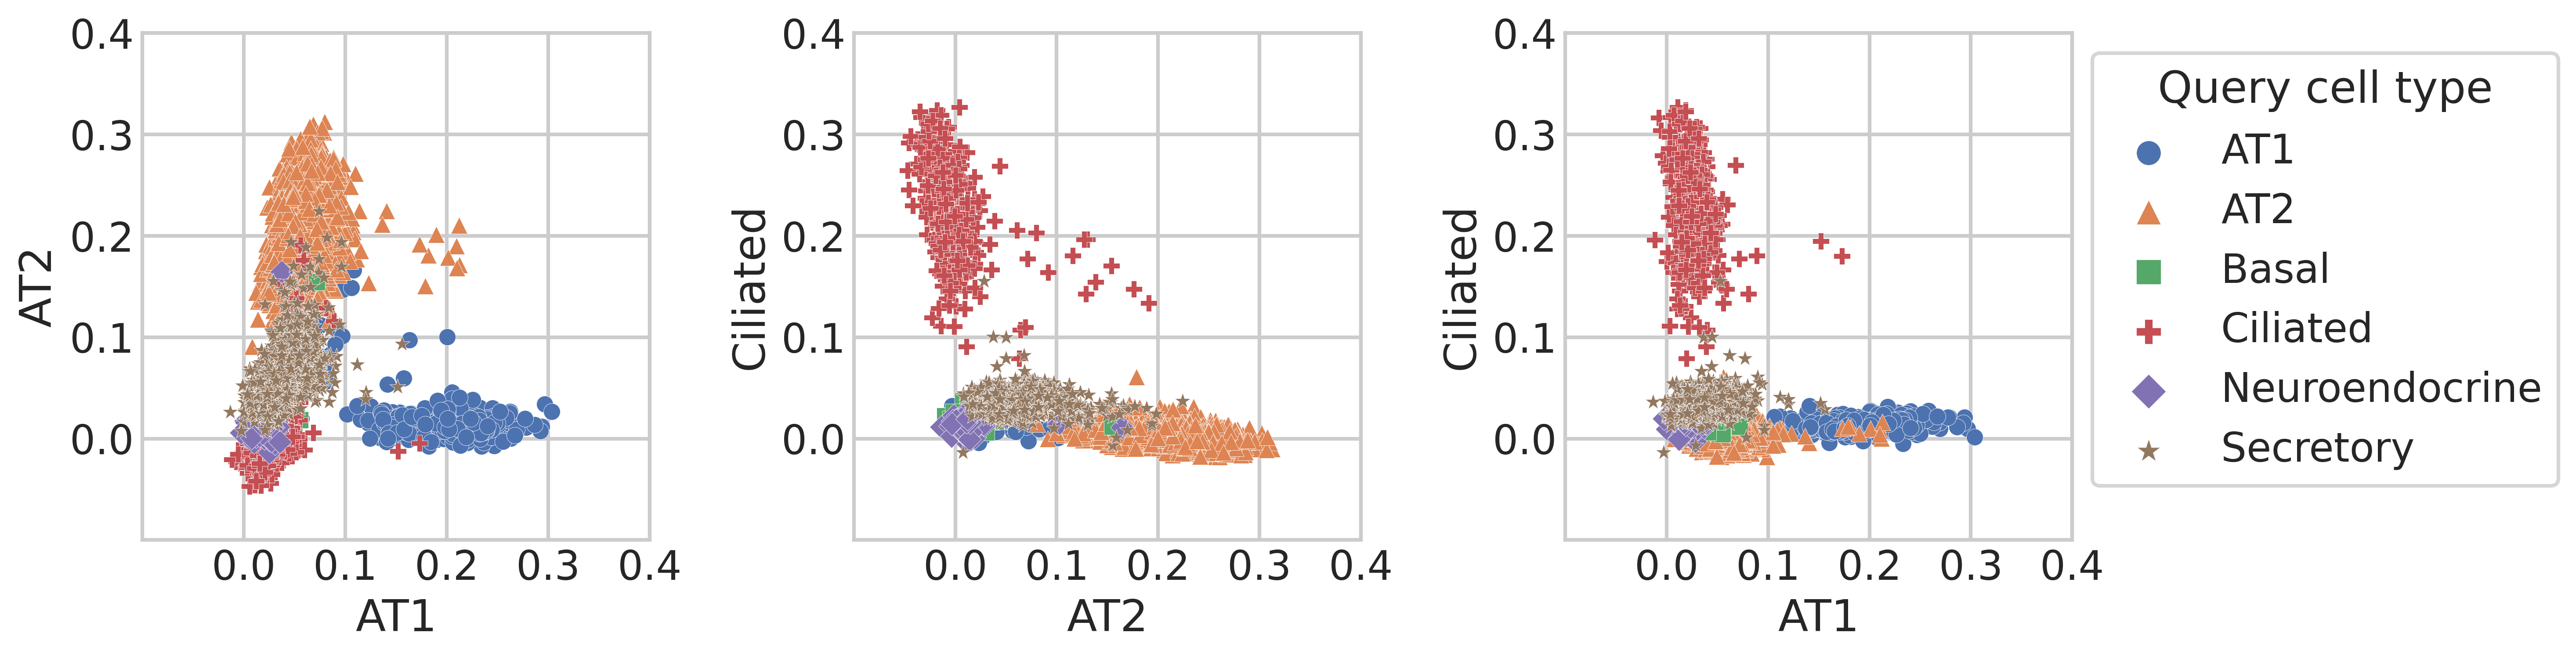
\includegraphics[scale=0.45]{figs/herriges colored by type.png}
        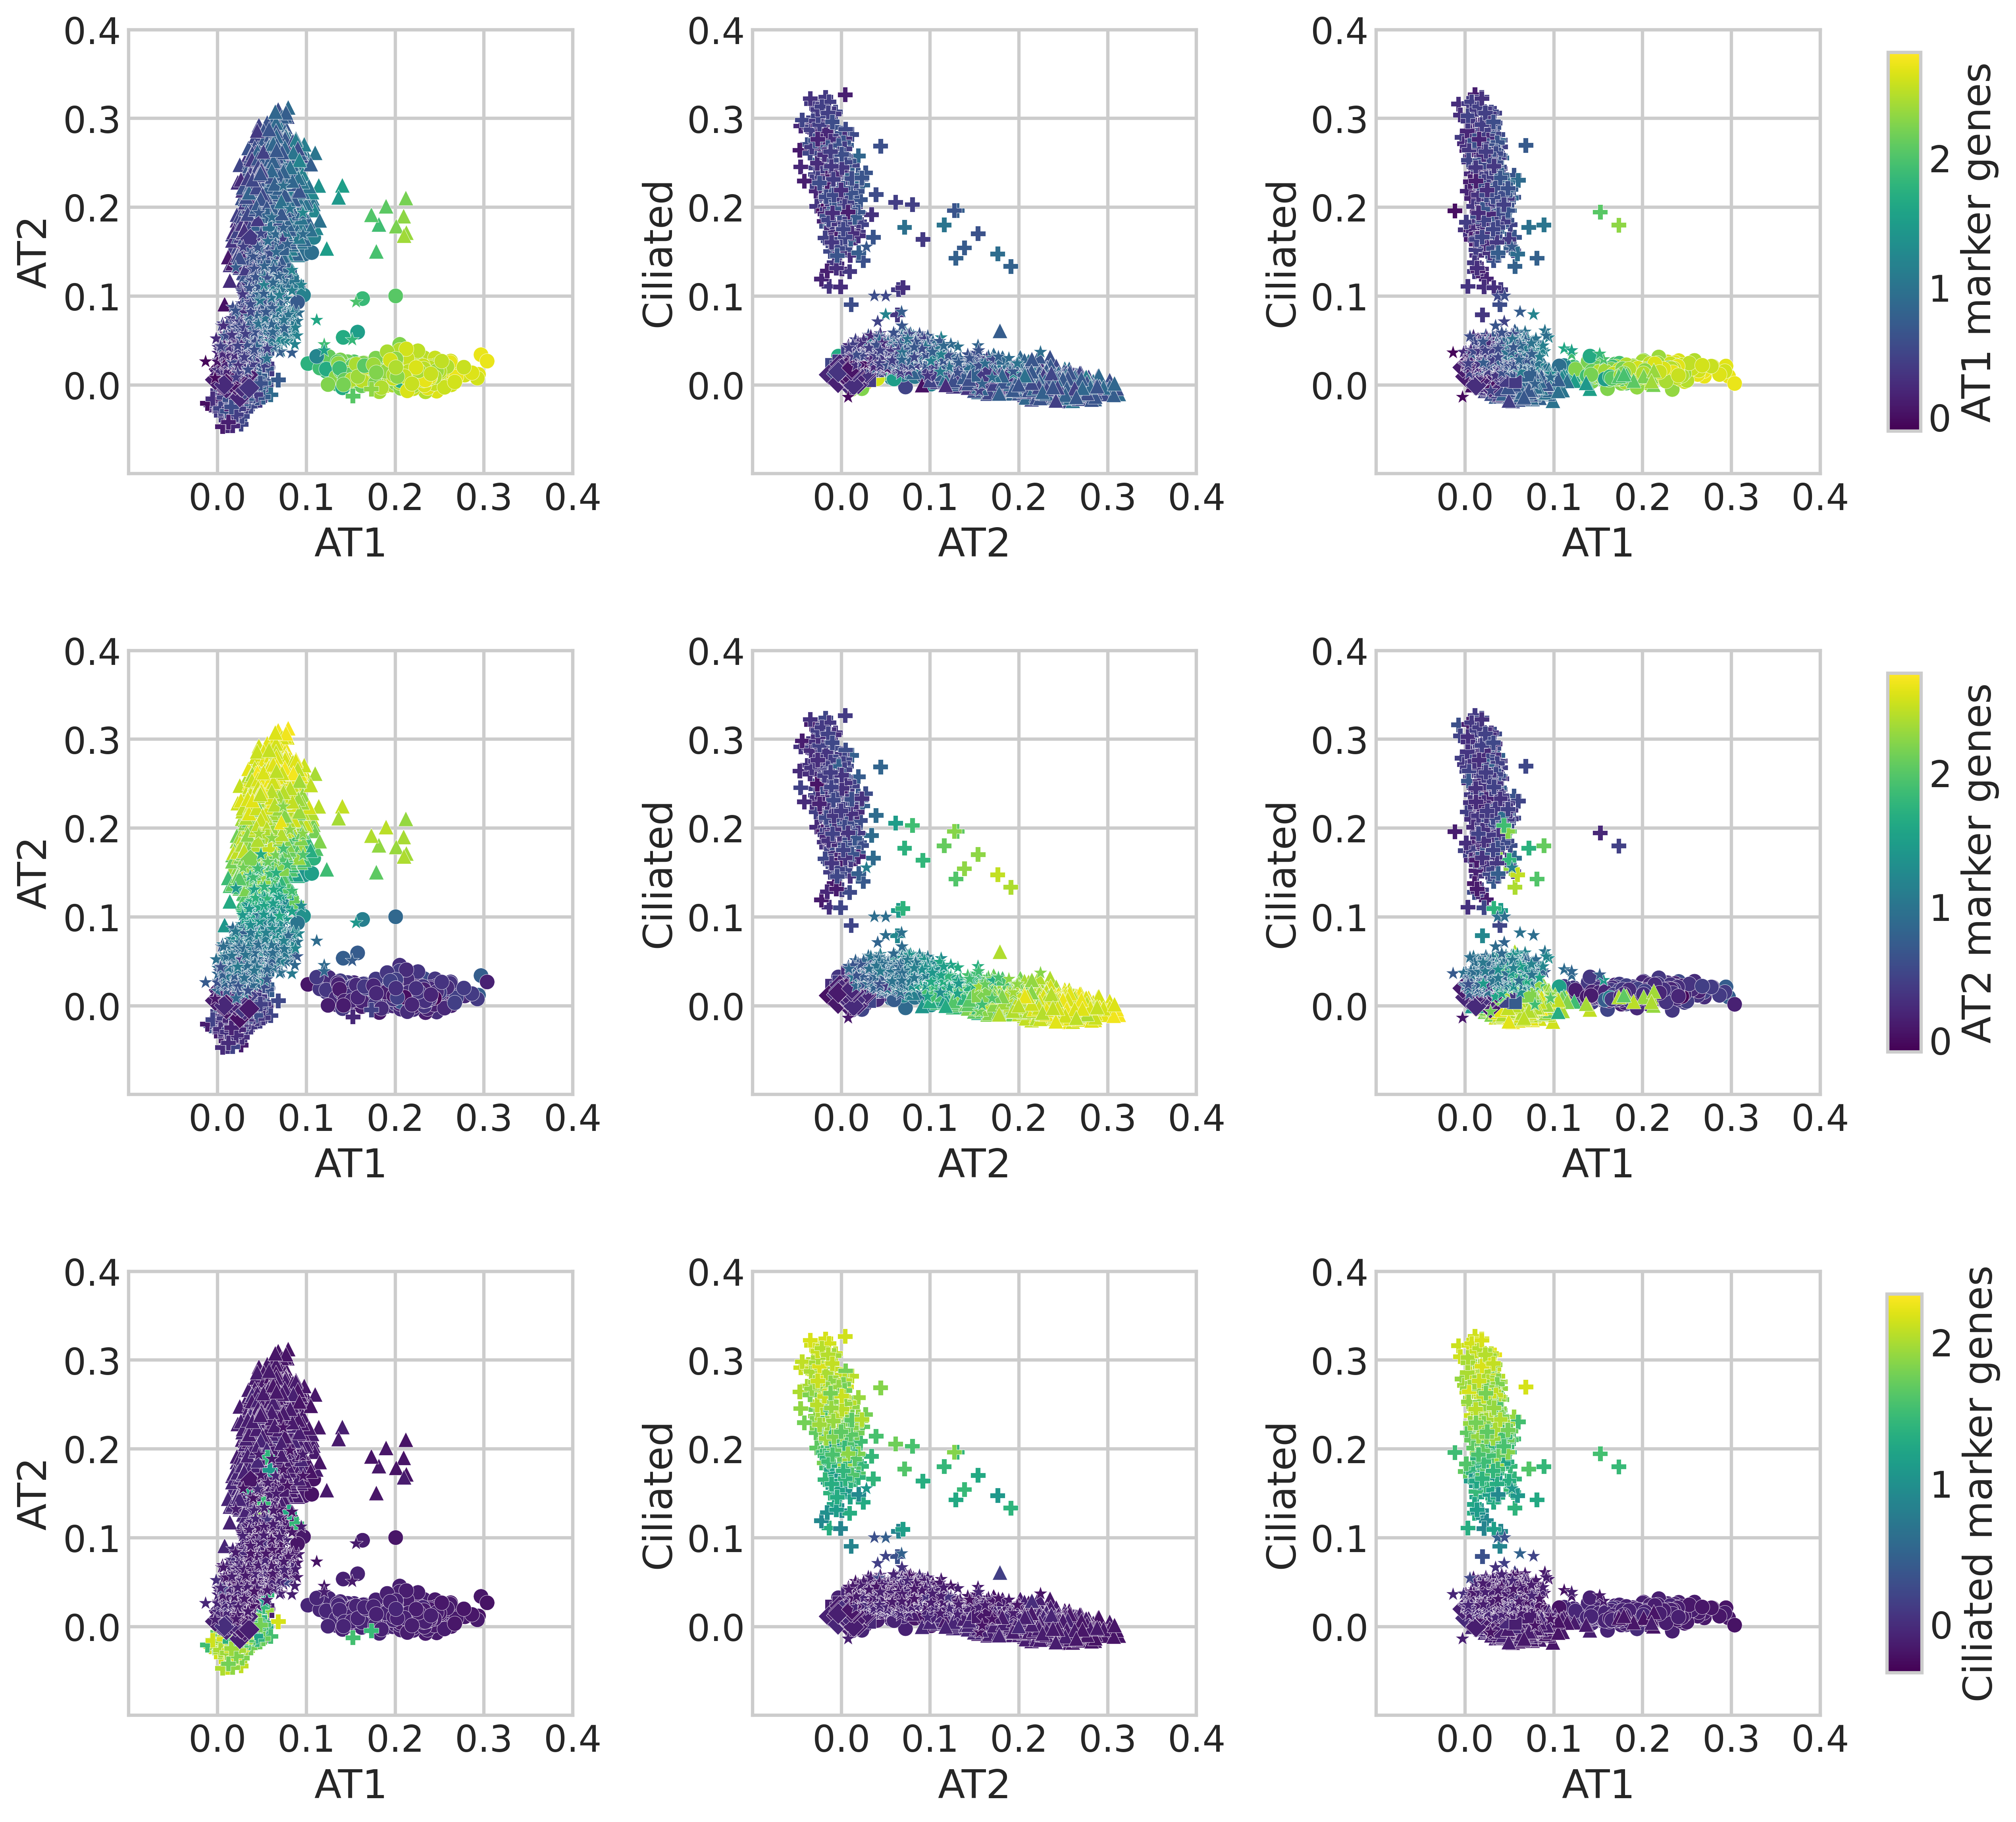
\includegraphics[scale=0.5]{figs/herriges colored by signature.png}
	\caption{scTOP identifies mouse lung cell types. Using the Mouse Cell Atlas as the reference basis, we show that mouse lung types separate clearly on scTOP score axes. The data points correspond to individual cells, and in the first row of plots, the marker shape and color indicate the "true type" as determined by annotations from Herriges et al. The axes used are scTOP scores for similarity with lung ciliated cells and alveolar types I and II. The second, third, and fourth rows of plots have individual cells colored by the marker genes for the type indicated by the color bars at the end of each row.}
	\label{herriges}
\end{figure}

\subsubsection{Example 2: Mouse Brain Atlas}

The mouse brain atlas\cite{yao_taxonomy_2021} sequenced over one million cells and clustered them into 42 subclasses and 101 supertypes. For a reference basis, we reserved a subset of 200 cells from each of the identified subclasses to use as training data. The test data, from which the accuracy score was calculated, was the remaining cells of each type not included in the training data. Ten different cell types are visualized in a grid in figure \ref{mouse_brain} (a). The color of each grid square corresponds to the average scTOP score of cells annotated as the type on the y-axis, with the cell type corresponding to the scTOP dimension on the x-axis. As shown by the distinct blue diagonal, the average scTOP score correctly matches the corresponding annotated cell type.

\begin{figure}
	\centering
    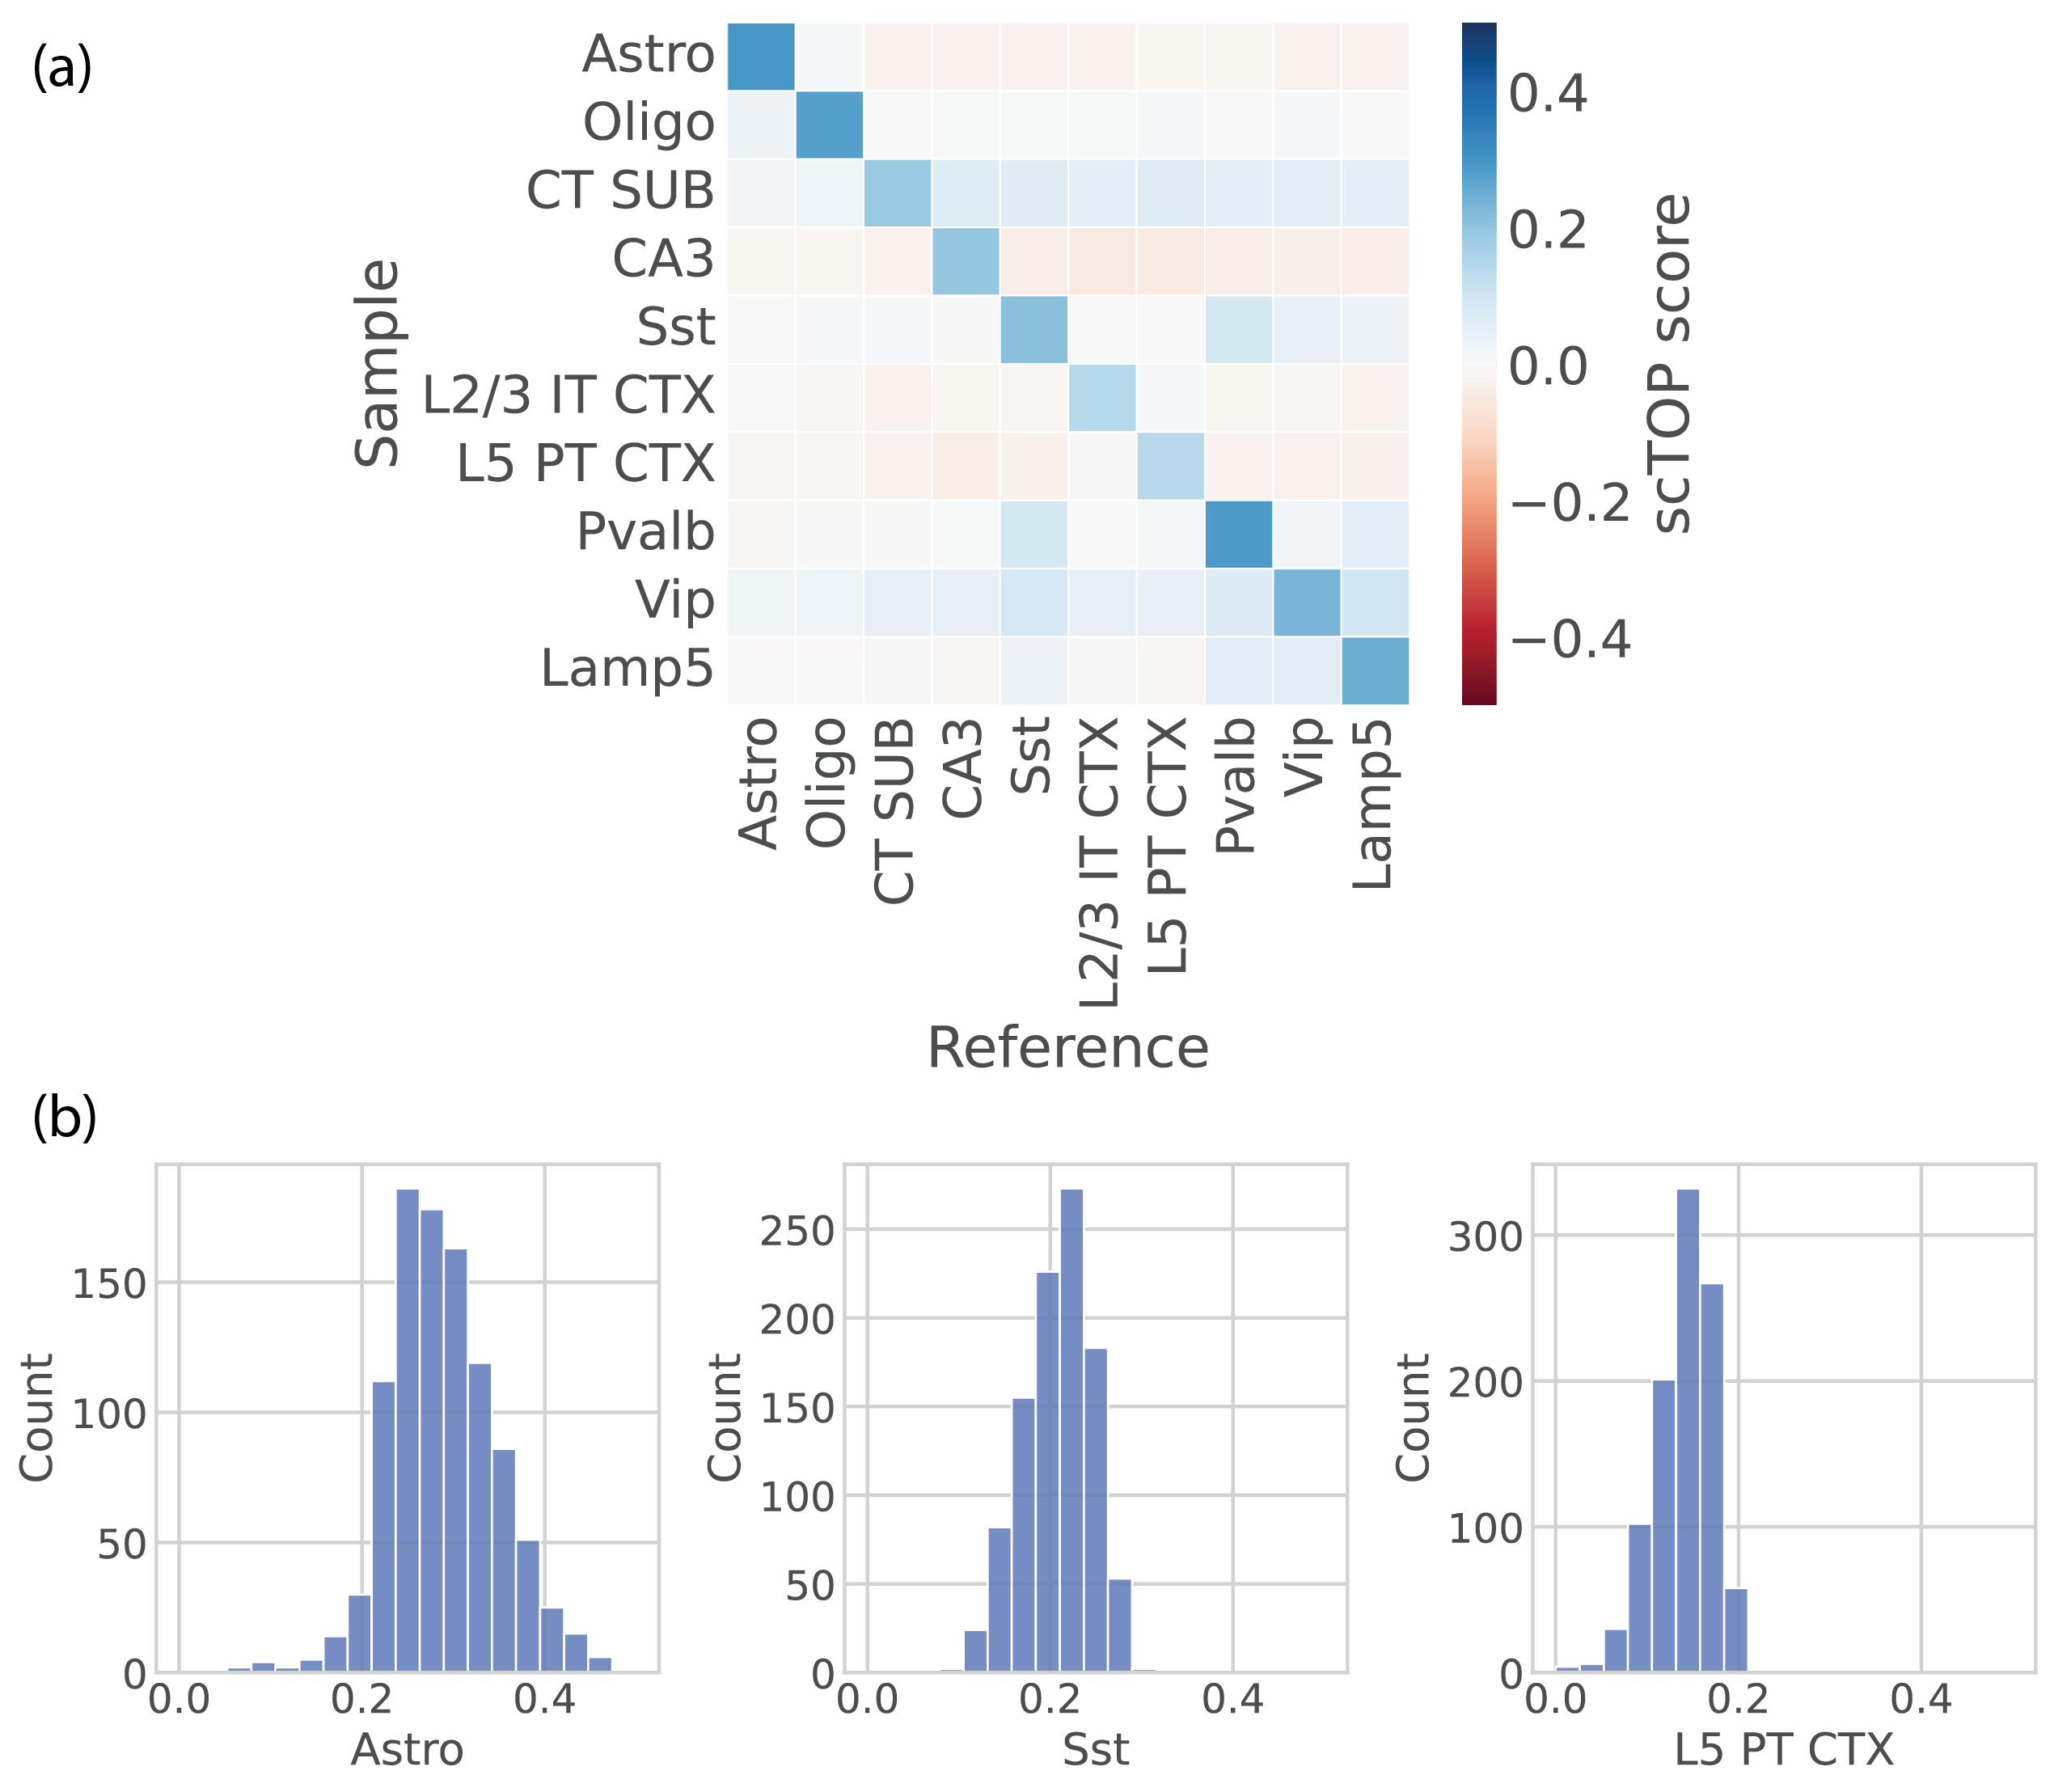
\includegraphics[scale=0.75]{figs/mouse brain.png}
	\caption{scTOP identifies mouse brain cell types. (a) Heatmap showing the average scTOP score for individual cells of the type indicated on the y-axis, compared to the reference types on the x-axis. A subset of cells from the Mouse Brain Atlas are used as the reference basis to query other cells from the same data set. The diagonal indicates that scTOP accurately matches query cells to the true reference type. (b) Histograms showing the distribution of scTOP scores for individual cells of the type labelling the x-axis. The scores shown are of the same type as the sample data. The far left histogram shows the distribtion of Astro scores for Astro cells, and the average of this distribution is indicated by the color of the upper left corner box in heatmap (a).}
	\label{mouse_brain}
\end{figure}

\subsubsection{Example 3: Matching cell types to tissues}

scTOP correctly identifies individual cells, and it can also identify the tissue to which a population of cells belongs. Instead of finding scTOP scores for individual cells, it's possible to group cells and average across them, then find the score for the averaged type. These aggregate pseudo-bulk scores tend to be higher than individual cell scores, since averaging over many cells compensates for the dropout effect. As shown in \ref{tabula_muris}, we found the aggregate scTOP scores for cells from the Mouse Cell Atlas projected onto the reference basis of Tabula Muris organs \cite{schaum_single-cell_2018}. Most cell types were correctly and strongly identified with the annotated tissue of origin. Parenchymal cell types were the most associated with the correct organ, while stromal cells were sometimes misidentified -- for example, the mammary gland endothelial cells. This is consistent with the fact that stromal cells are less specified to each organ. A discussion of the accuracy of scTOP when applied to stromal types versus parenchymal types may be found in appendix \ref{failure_cases}.

\begin{figure}
	\centering
    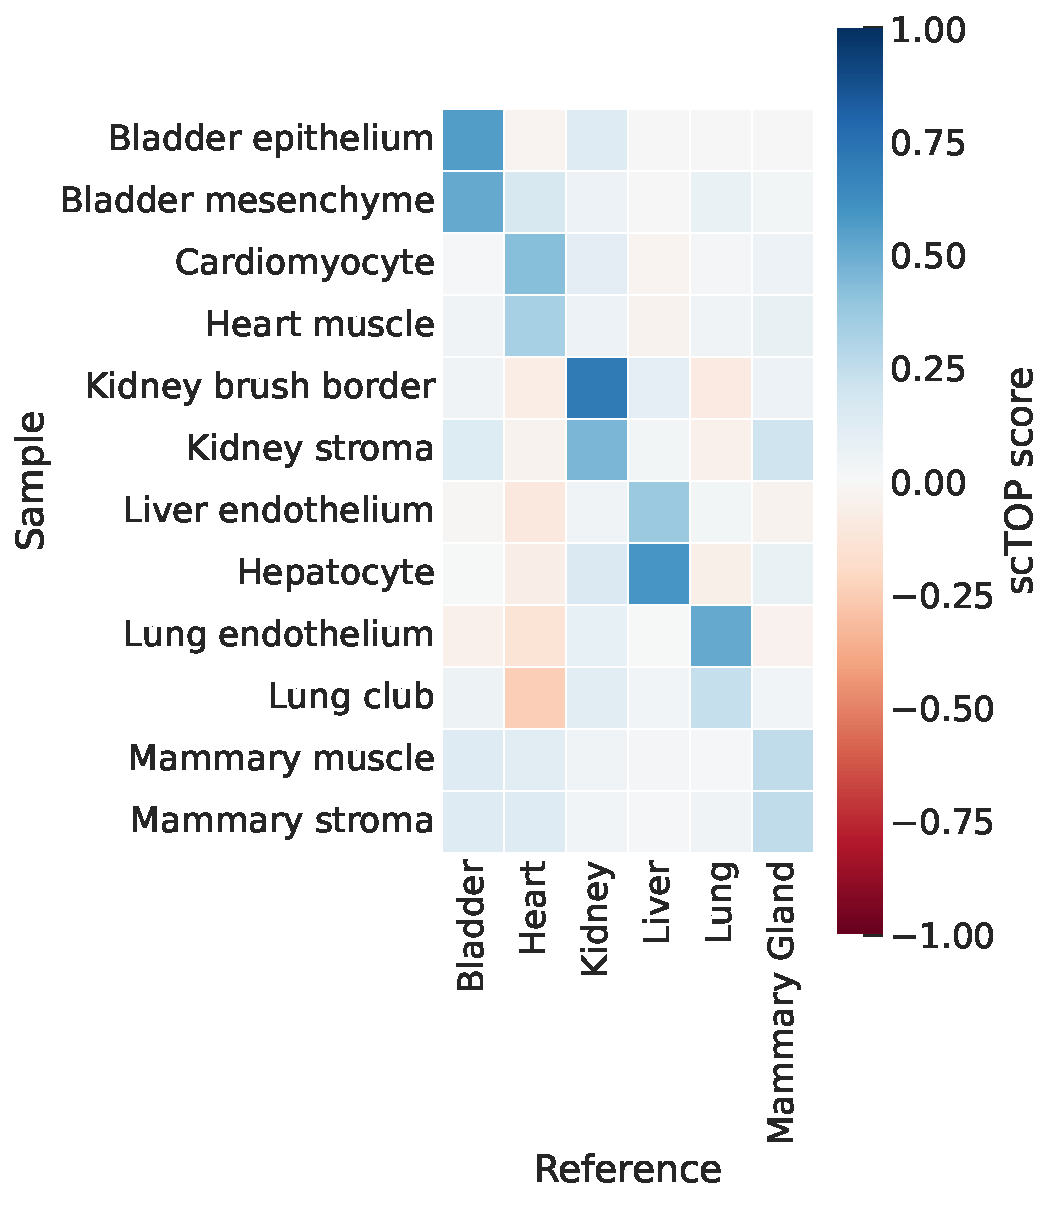
\includegraphics[scale=0.5]{figs/tabula muris heatmap.pdf}
	\caption{scTOP is able to classify tissues at different resolutions. Aggregate pseudo-bulk samples from the Mouse Cell Atlas are compared to a reference basis consisting of organs from Tabula Muris. The scTOP scores are significantly higher when comparing a cell type with the organ of origin. The shade of each bin indicates the average scTOP score for an individual queried cell compared to the cell type indicated on the x-axis. The y-axis lists the true types of the queried cells. The dark diagonal demonstrates the scTOP scores correctly match the queried data to the corresponding true types.}
	\label{tabula_muris}
\end{figure}

\subsubsection{Example 4:  Human data}

The CellBench dataset \cite{tian_benchmarking_2019} was designed specifically to benchmark scRNA-seq analysis methods. We used the subset of data pertaining to five cancer lines. 200 cells from each line were used as training data to create the reference basis, then the rest of the cells were input as query data. As shown in figure \ref{cellbench} and table \ref{table:1}, scTOP classifies cell line identity of the test data with 100 percent accuracy. 

\begin{figure}
	\centering
		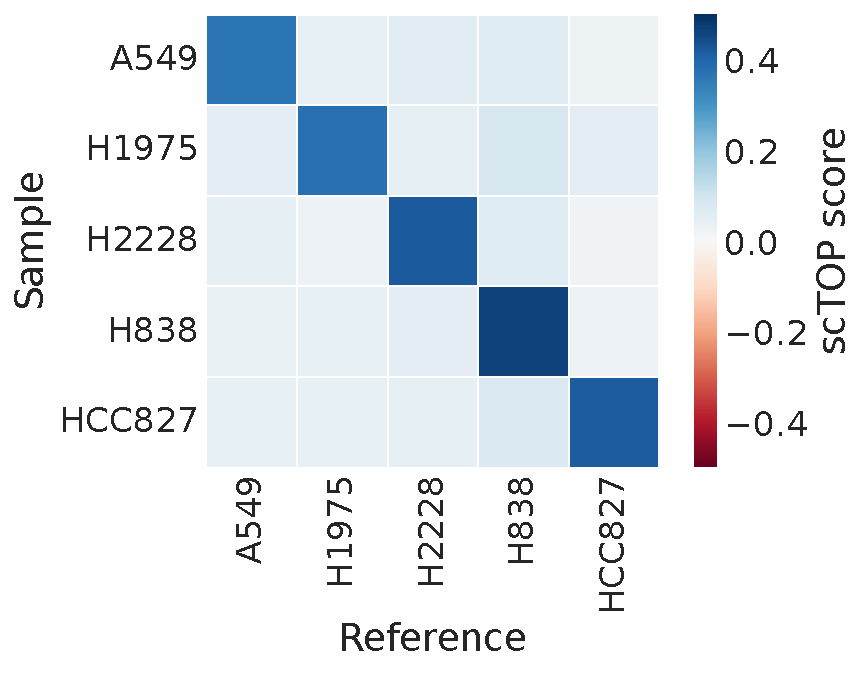
\includegraphics[scale=0.5]{figs/cellbench heatmap.pdf} 
	\caption{scTOP correctly identifies human tissues. The CellBench data set contains human cell cancer lines specifically processed to serve as benchmarking for scRNA-seq algorithms. We take a subset of cells to use as the reference basis in analyzing the rest of the CellBench data. The shade of each bin indicates the average scTOP score for an individual queried cell compared to the cell type indicated on the x-axis. The y-axis lists the true types of the queried cells. The dark diagonal demonstrates the scTOP scores correctly match the queried data to the corresponding true types.}
	\label{cellbench}
\end{figure}

To further prove the power of scTOP in classifying human samples, we analyzed data from the human lung atlas dataset \cite{travaglini_molecular_2020}. This dataset sequenced thousands of human lung cells and identified 58 phenotypic popoulations. For our analysis, we restricted the training and test data to epithelial and stromal types that had at least 200 cells in each type population. The reference basis was created using 80\% of the cells from each population, and the query data consisted of the remaining 20\% of the data. Figure \ref{human lung} shows that the scTOP scores were consistently high in cases where the score type matched the true type of the query.

\begin{figure}
	\centering
		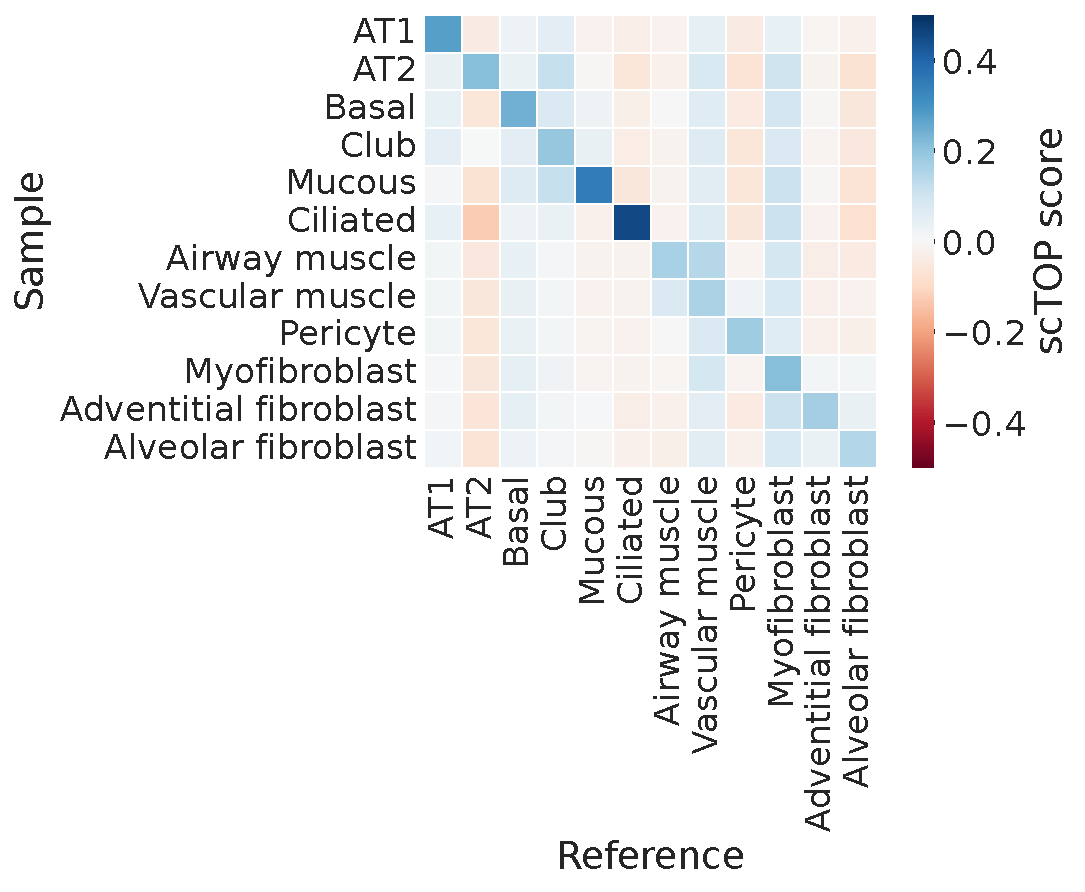
\includegraphics[scale=0.5]{figs/human lung heatmap.pdf}
	\caption{scTOP correctly identifies human tissues. Similar to figure \ref{cellbench}, cells from the Human Lung Atlas are compared to a reference basis constructed from cells from the Human Lung Atlas. The colors of the bins correspond to average scTOP scores of individual cells. Again, the diagonal is the most prominent section, showing that cells of the y-axis types are correctly matched to the reference x-axis identities.}
	\label{human lung}
\end{figure}

As demonstrated by the diverse data sources examined here, as long as a well-defined reference basis is available, scTOP works extremely well  for cell type identifciation across different measurement conditions, species, organs, and resolutions. This performance is especially impressive since as discussed earlier, the algorithm does not use dimensional reduction methods such as PCA, tSNE, UMAP, or SPRING, or make use of any statistical fitting procedures.

\subsection{Tracking cell type transitions}

{\color{red}: PM: This section needs to be revisited once figures are finalized}

We now illustrate how scTOP can be used to visualize developmental dynamics directly in cell type space. 

\subsubsection{Lung development}
The healthy formation of lungs is vital to mammalian life. For a mammal to breathe and live independently after birth, the final stages of embryonic development must equip it with the ability to exchange gases with its environment. Zepp et al. [CITE] sought to examine the formation of pulmonary alveoli, small sacs where oxygen and carbon dioxide are transferred between the lungs and the air, in the developing mouse. They sequenced mouse lungs between post-conception day 12.5 (E12.5) and postnatal day 42 (P42). As shonw in figure \ref{LungMAP}, we found the scTOP scores for cells annotated by Zepp et al. as type I pneumocytes, type II pneumocytes, and epithelial progenitor cells. The reference basis consisted of adult cell types from the Mouse Cell Atlas and an E12 epithelial progenitor cell type from the Atlas of Lung Development \cite{negretti_single-cell_2021}.

Figure 1I from Zepp et al. conjectures that one begins to see separate alveolar type 1 and type 2 populations between E15.5 and E17.5. According to our plot, at those days there are populations of cells clearly headed towards the two types. There is also a population of cells in between expressing both type 1 and type 2 signatures. Zepp et al. propose these cells are a transitional state similar to the Axin2+ state described by Frank et al. [CITE]. However, as shown in figure \ref{LungMAP genes} (a), the AT1/AT2 cells are not significantly expressing Axin2+. Verheyden and Sun [CITE] summarize the variety of previously-described transitional AT1/AT2 states: alveolar differentiation intermediate (ADI) [CITE Strunz], pre-alveolar type-1 transitional cell state (PATS) [CITE Kobayashi], and damage-associated transient progenitors (DATPs) [CITE Choi]. None of the relevant marker genes for those states were significantly more expressed in the AT1/AT2 cells than either or both of the AT1 or AT2 clusters (figure \ref{LungMAP genes} (b) - (d)). Performing differential gene analysis on the clusters also failed to identify any genes that were uniquely expressed in the AT1/AT2 cluster, indicating the cells in this population are truly in a mixed state.

Because scTOP provides us with reference axes that don't change according to whatever data is included, it is possible to track different data points across time on the same axes. These axes are also easily interpretable: they measure the similarity to a known cell type.

\begin{figure}
	\centering
		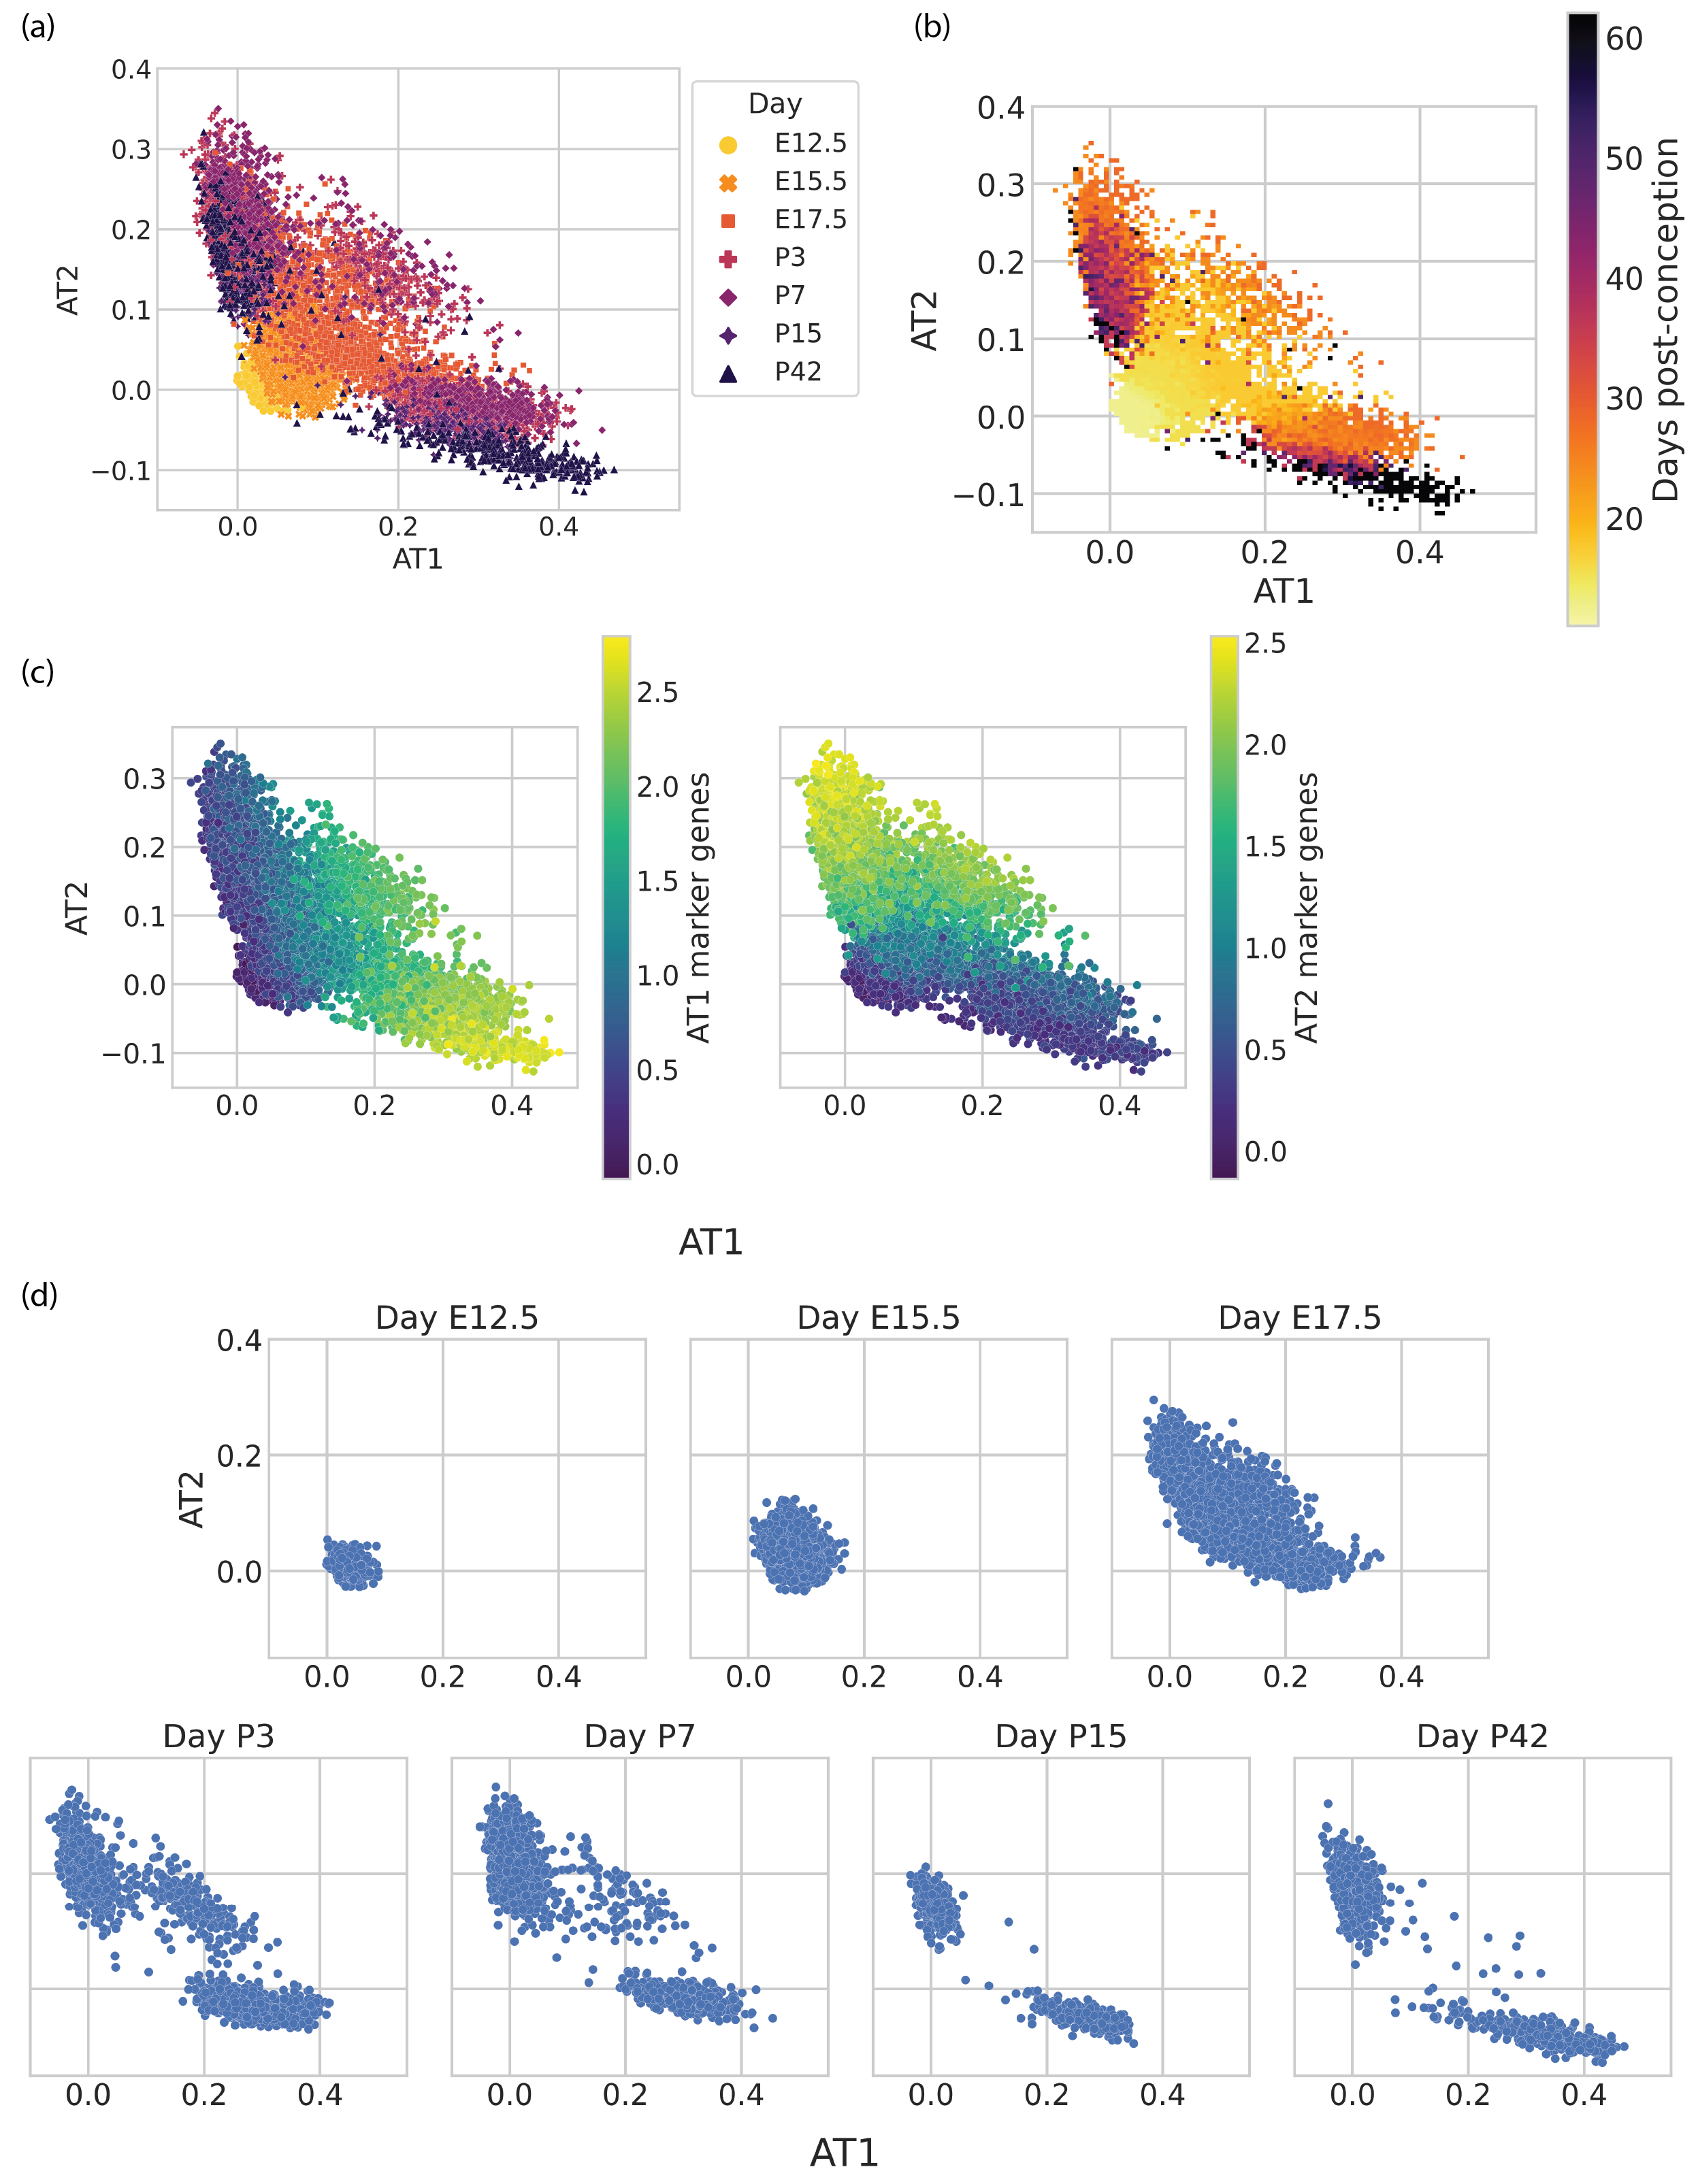
\includegraphics[scale=0.7]{figs/LungMAP.png}
	\caption{Visualizing the developing mouse lung with scTOP. (a) scTOP illustrates specification of alveolar type I and type II cells in murine embryonic development. Alveolar cells from Zepp et al. are compared to a reference basis constructed from adult lung cells from Herriges et al. and early epithelial cells from the Atlas of Lung Development. The color and shape of each data point indicates the age of the mouse embryo from which the sample was extracted, from post-conception day 12,5 (E12.5) to 42 days post-birth (P42). (b) The same data as in (a) is displayed as a 2D histogram, with each bin colored corresponding to the average day of the data point(s) falling within that bin. The color trend shows that early cells generally have very low AT1 and AT2 scores, then the AT1 and AT2 scores increase over time.  (c) Scatter plots of the same data as in (a) and (b), now colored by the average expression of AT1 markers genes (left) and AT2 marker genes (right). The scTOP scores of AT1 (AT2) cells are high when the average AT1 (AT2) marker gene expression is high. (d) Scatter plots showing the same data as in the above plots, separated by day to show the combination AT1/AT2 population is most apparent at days P3 and P7.}
	\label{LungMAP}
\end{figure}

\subsubsection{Visualizing hematopoiesis using lineage tracing data}

The case of a general cell type differentiating into mature types is exemplified by the case of hematopoiesis, the process of blood regeneration that takes place in bone marrow. In this process, the progenitor is the hematopoietic stem cell, which may become one of a number of blood types such as megakaryocyte, erythrocyte, monocyte, etc. It is unknown what causes a hematopoietic stem cell to end up in one fate or another; perhaps it is due to small differences in the epigenetic landscape when the stem cells are dividing, or perhaps it is due to small differences in signals the cells receive over time. Weinreb et al. \cite{weinreb_lineage_2020} sought to answer this question using a combination of scRNA-seq and lineage tracing. Since cells are destroyed when they are sequenced, it isn't possible to repeatedly sequence the same cell to watch it differentiate over time. As a substitute for watching one cell develop, there are various methods of tracing the lineage of a cell by sequencing clones and observing the gene expression levels of clones. Weinreb et al. created a tool for lineage and RNA recovery (LARRY) and applied it to hematopoiesis in mice. By tagging cells with DNA barcodes then letting them multiply, they were able to use scRNA-seq to identify clone sisters across generations of cell division.

To apply LARRY to blood cells, they extracted hematopoietic progenitor cells from mice, barcoded the cells, waited for the progenitors to multiply in primary culture, then performed scRNA-seq at days 2, 4, and 6 post-barcoding. Then, they extracted blood cells at four and six days in cultre. The resulting dataset contains over 300,000 cells, with 2,632 clones spanning time points. Clones belonging to the same clonal family are referred to as "sisters." They then used pseudotime orderings to identify a transcriptomic map to identify lienages of the cells. This map used transcriptomic similarity to place the individual cells accoridng to "pseudotime". With scTOP, creating a pseudotime ordering is unnecessary. Instead of arranging cells according to transcriptomic similarity to one another using a dimensional reduction method (what method did they use??), we used scTOP to compare clones to day 2 undifferentiated cells and day 6 mature cell types. We used the annotations from Weinreb et al. to identify these populations. The resulting reference basis consisted of day 2 undifferentiated progenitors and day 6 neutrophils, monocytes, megakaryocytes, mast cells, eosiniphils, and basophils. 

We found scTOP scores for clonal families with sisters that spanned multiple days. The scores for the undifferentiated hematopoietic progenitor stem cell decreased over time, while the scores for the mature types increased. Figure \ref{hem clones}, shows these changes through time for three clonal families. 

The clonal family in figure \ref{hem clones} (a) ended up with some sisters that are neutrophils and some that are monocytes. As time passes and the cells mature, their scores for neutrophil and monocytes increase. The graph with neutrophils on the horizontal axis and monocytes on the vertical axis shows that one subset of the population moved towards high-monocyte, low-neutrophil score and the other subset moved towards low-monocyte, high-neutrophil. This indicates that the same progenitor cell can result in either monocytes or neutrophils. 

scTOP can reveal differentiation pathways without the need for pseudotime inference. Pseudotime inference and other dimensional reduction methods place cells next to one another, which can bias results. It's difficult to draw conclusions about certain genes being expressed at different points in pseudotime; patterns may arise that suggest a continuous progression of differentiation, but the progression may be the result of an algorithm inferring that cells which express similar genes should be next to one another in pseudotime, creating a progression by assumption. scTOP avoids this issue by comparing cells to a reference instead of grouping them by similarity to one another. Weinreb et al. claim that the dimensional reduction shown in figure 4 (a) indicates there are two pathways of monocyte differentiation, one that expresses dendritic cell markers and one that expresses neutrophil markers. We used scTOP to visualize all the in vitro clones in terms of similarity to neutrophils, monocytes, and progenitors (\ref{hem genes}). This allows us to see which cells are more likely to be neutrophils that exhibit some monocyte-like genes rather than neutrophil-like monocytes. However, one limitation of scTOP is that it requires sufficient cells to create a reliable reference from; since there were too few dendritic cells to serve as reference, it was not possible to calculate dendritic cell scores.

While figure \ref{FIG:5}a shows scTOP scores for one clonal family, figure \ref{FIG:5}b shows a 2-dimensional histogram of scTOP scores for all of the multi-generational clonal families. The horizontal axes on these plots indicate the "undifferentiated" score while the vertical axes indicate all of the mature cell types included in the reference basis. Each bin of the 2-dimensional histogram is colored according to the average day of all the cells that fall within that bin; although the cells were only sampled at days 2, 4, and 6, the bin time points form a continuous range because they are averages of varying quantities of day 2, 4, and 6 cells. These plots show that, as expected, the day 2 cells generally have high "undifferentiated" scores, which decrease over time. As time passes, the scores corresponding to a given differentiated cell type increase or remain at zero, since some clones end up at that particular type and some end up at another type. 

Figure \ref{FIG:5}c shows 2D histograms for differentiated type scores compared to other differentiated type scores. One can see that differentiation pathways for some cell types are mutually suppressive while others form a continuous spectrum between identities. For example, megakaryocytes and monocytes form a distinct L-shape that indicates the development program for each of these types prevents the program of the other; cells are either megakaryocytes, monocytes, or neither, there is no in-between stage. However, the plot for monocytes and neutrophils tells a different story: instead of having a distinct L-shape with narrow distribution along the axes, this plot shows a continuous spectrum of cells that are monocyte-like, neutrophil-like, and every step in-between. 

{\color{red} PM: We need 3-4 paragraphs discussing our biological results. For example, what lineages to single clones end up at together, which don't they... Then, we also need to place our conclusions in context of original paper -- and ideally what other biology is known... Like they emphasize this transition cells or whatever See Figure 4 of theirs and Ref 27 they dialogue with . }

\begin{figure}
	\centering
		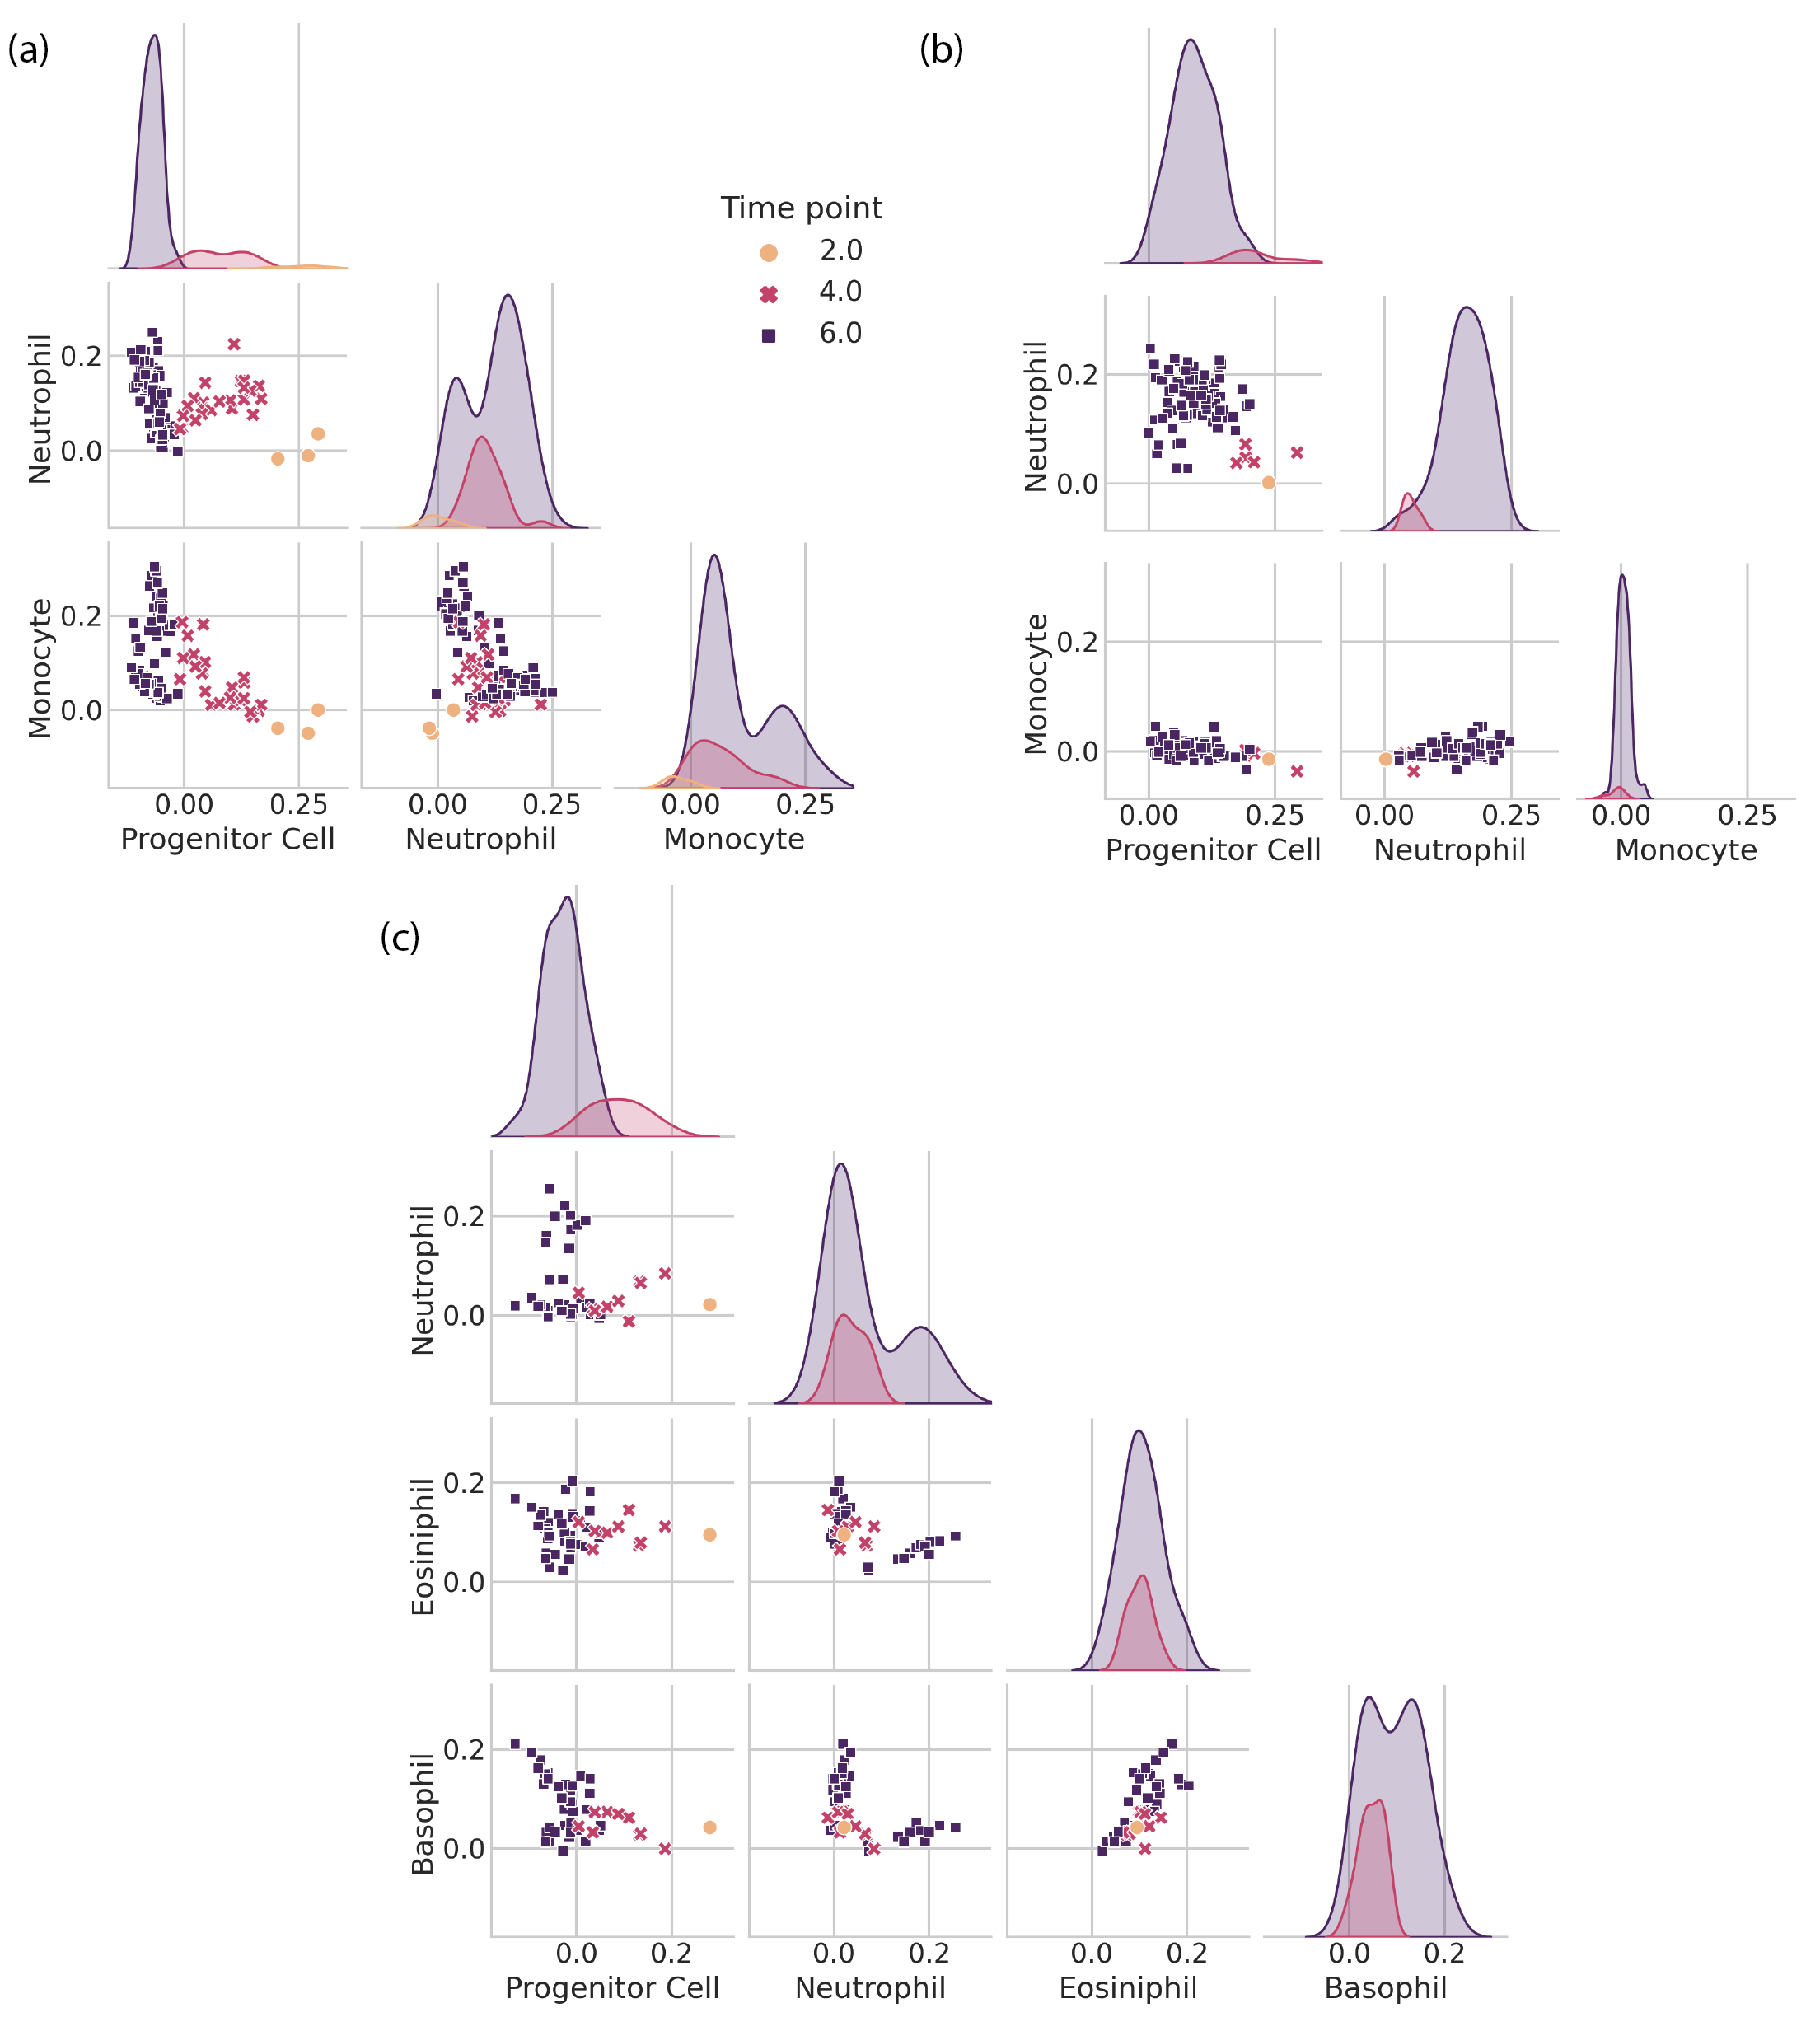
\includegraphics[scale=0.75]{figs/hem. clone families.png}
	\caption{Tracing hematopoietic cells differentiation with scTOP. (a), (b), (c) display scatter plots and distributions of scTOP scores for individual in vitro clone families from Weinreb et al. The scatter plots show the x-axis scTOP score compared to the y-axis scTOP score for individual cells, while the distributions show the scTOP scores of the type indicated on the x-axis of the corresponding column. The color and shape of each marker (and color of each distribution) indicate the days in culture at which the cells were extracted. (a) A clone family where some clones end up becoming neutrophils and some become monocytes. At day 2, the 3 sister cells have low neutrophil and monocyte scores, and high progenitor scores. At days 4 and 6, the progenitor scores decrease and a portion of the cells increase in monocyte scores while others increase in neutrophil scores. (b) A clone family where all of the cells end up becoming neutrophils. (c) A clone family where the descendant cells become neutrophils, eosiniphils, and basophils.}
	\label{hem clones}
\end{figure}


\begin{figure}
	\centering
		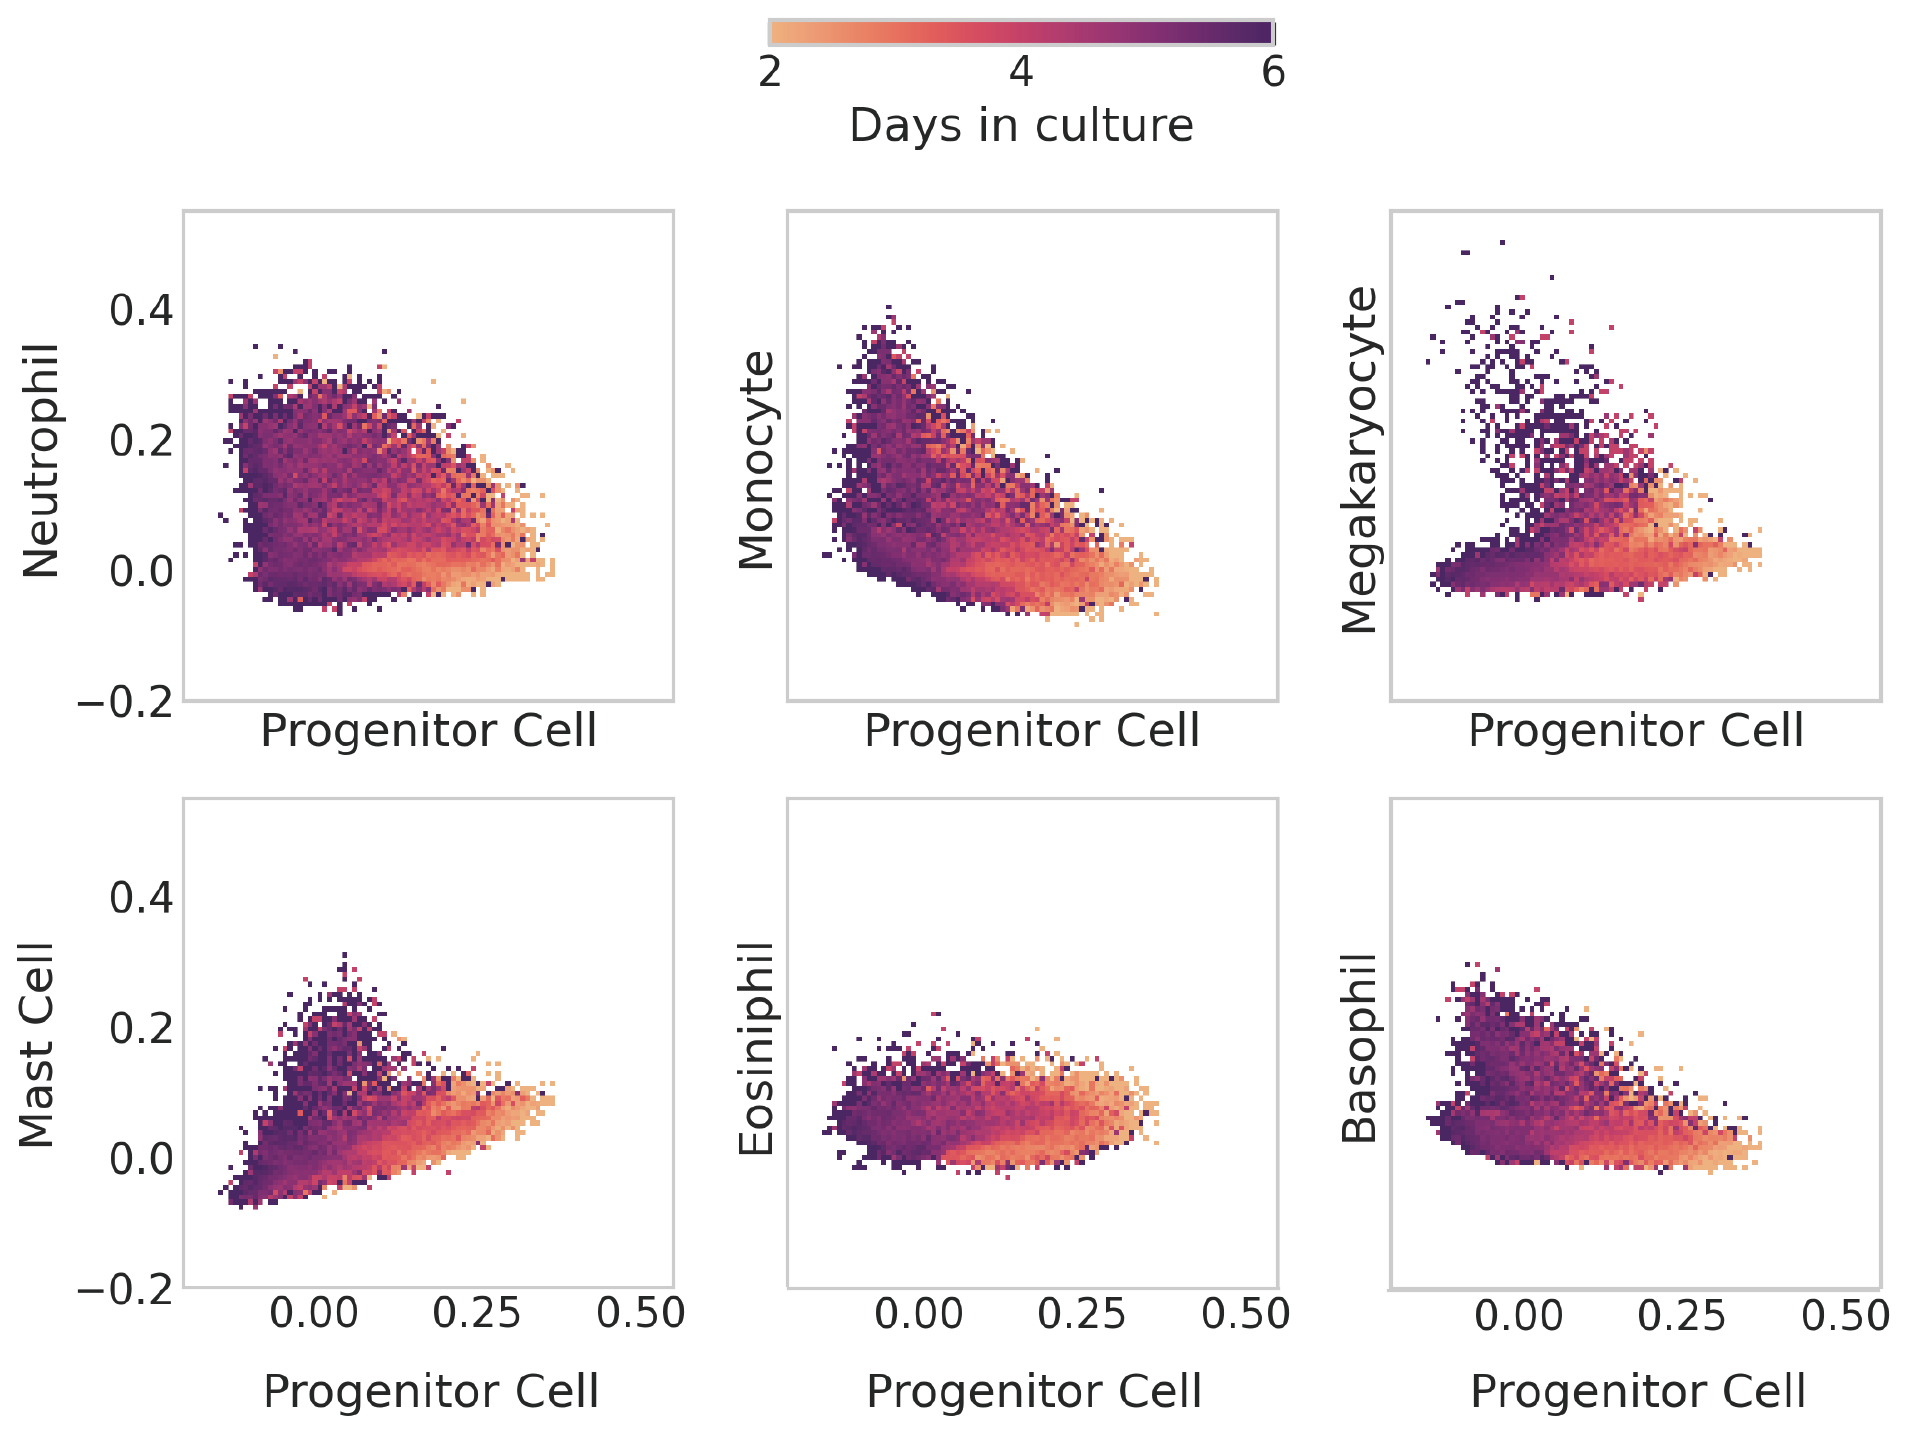
\includegraphics[scale=0.75]{figs/hem progenitor hists.png}
	\caption{Tracing differentiation of hematopoietic cells from progenitor to mature type. The plots shown here are 2D histograms of all of the in vitro clone families from Weinreb et al., with the x-axis of each one indicating the scTOP score for hematopoietic progenitor type and the y-axis showing the score for a mature type. Each bin of the histogram is colored by the average day in culture of the data points that fall within the bin. Early cells have high progenitor scores and low mature type scores. As time passes cells end up with high scores in mature types.}
	\label{hem progenitor}
\end{figure}

\begin{figure}
	\centering
		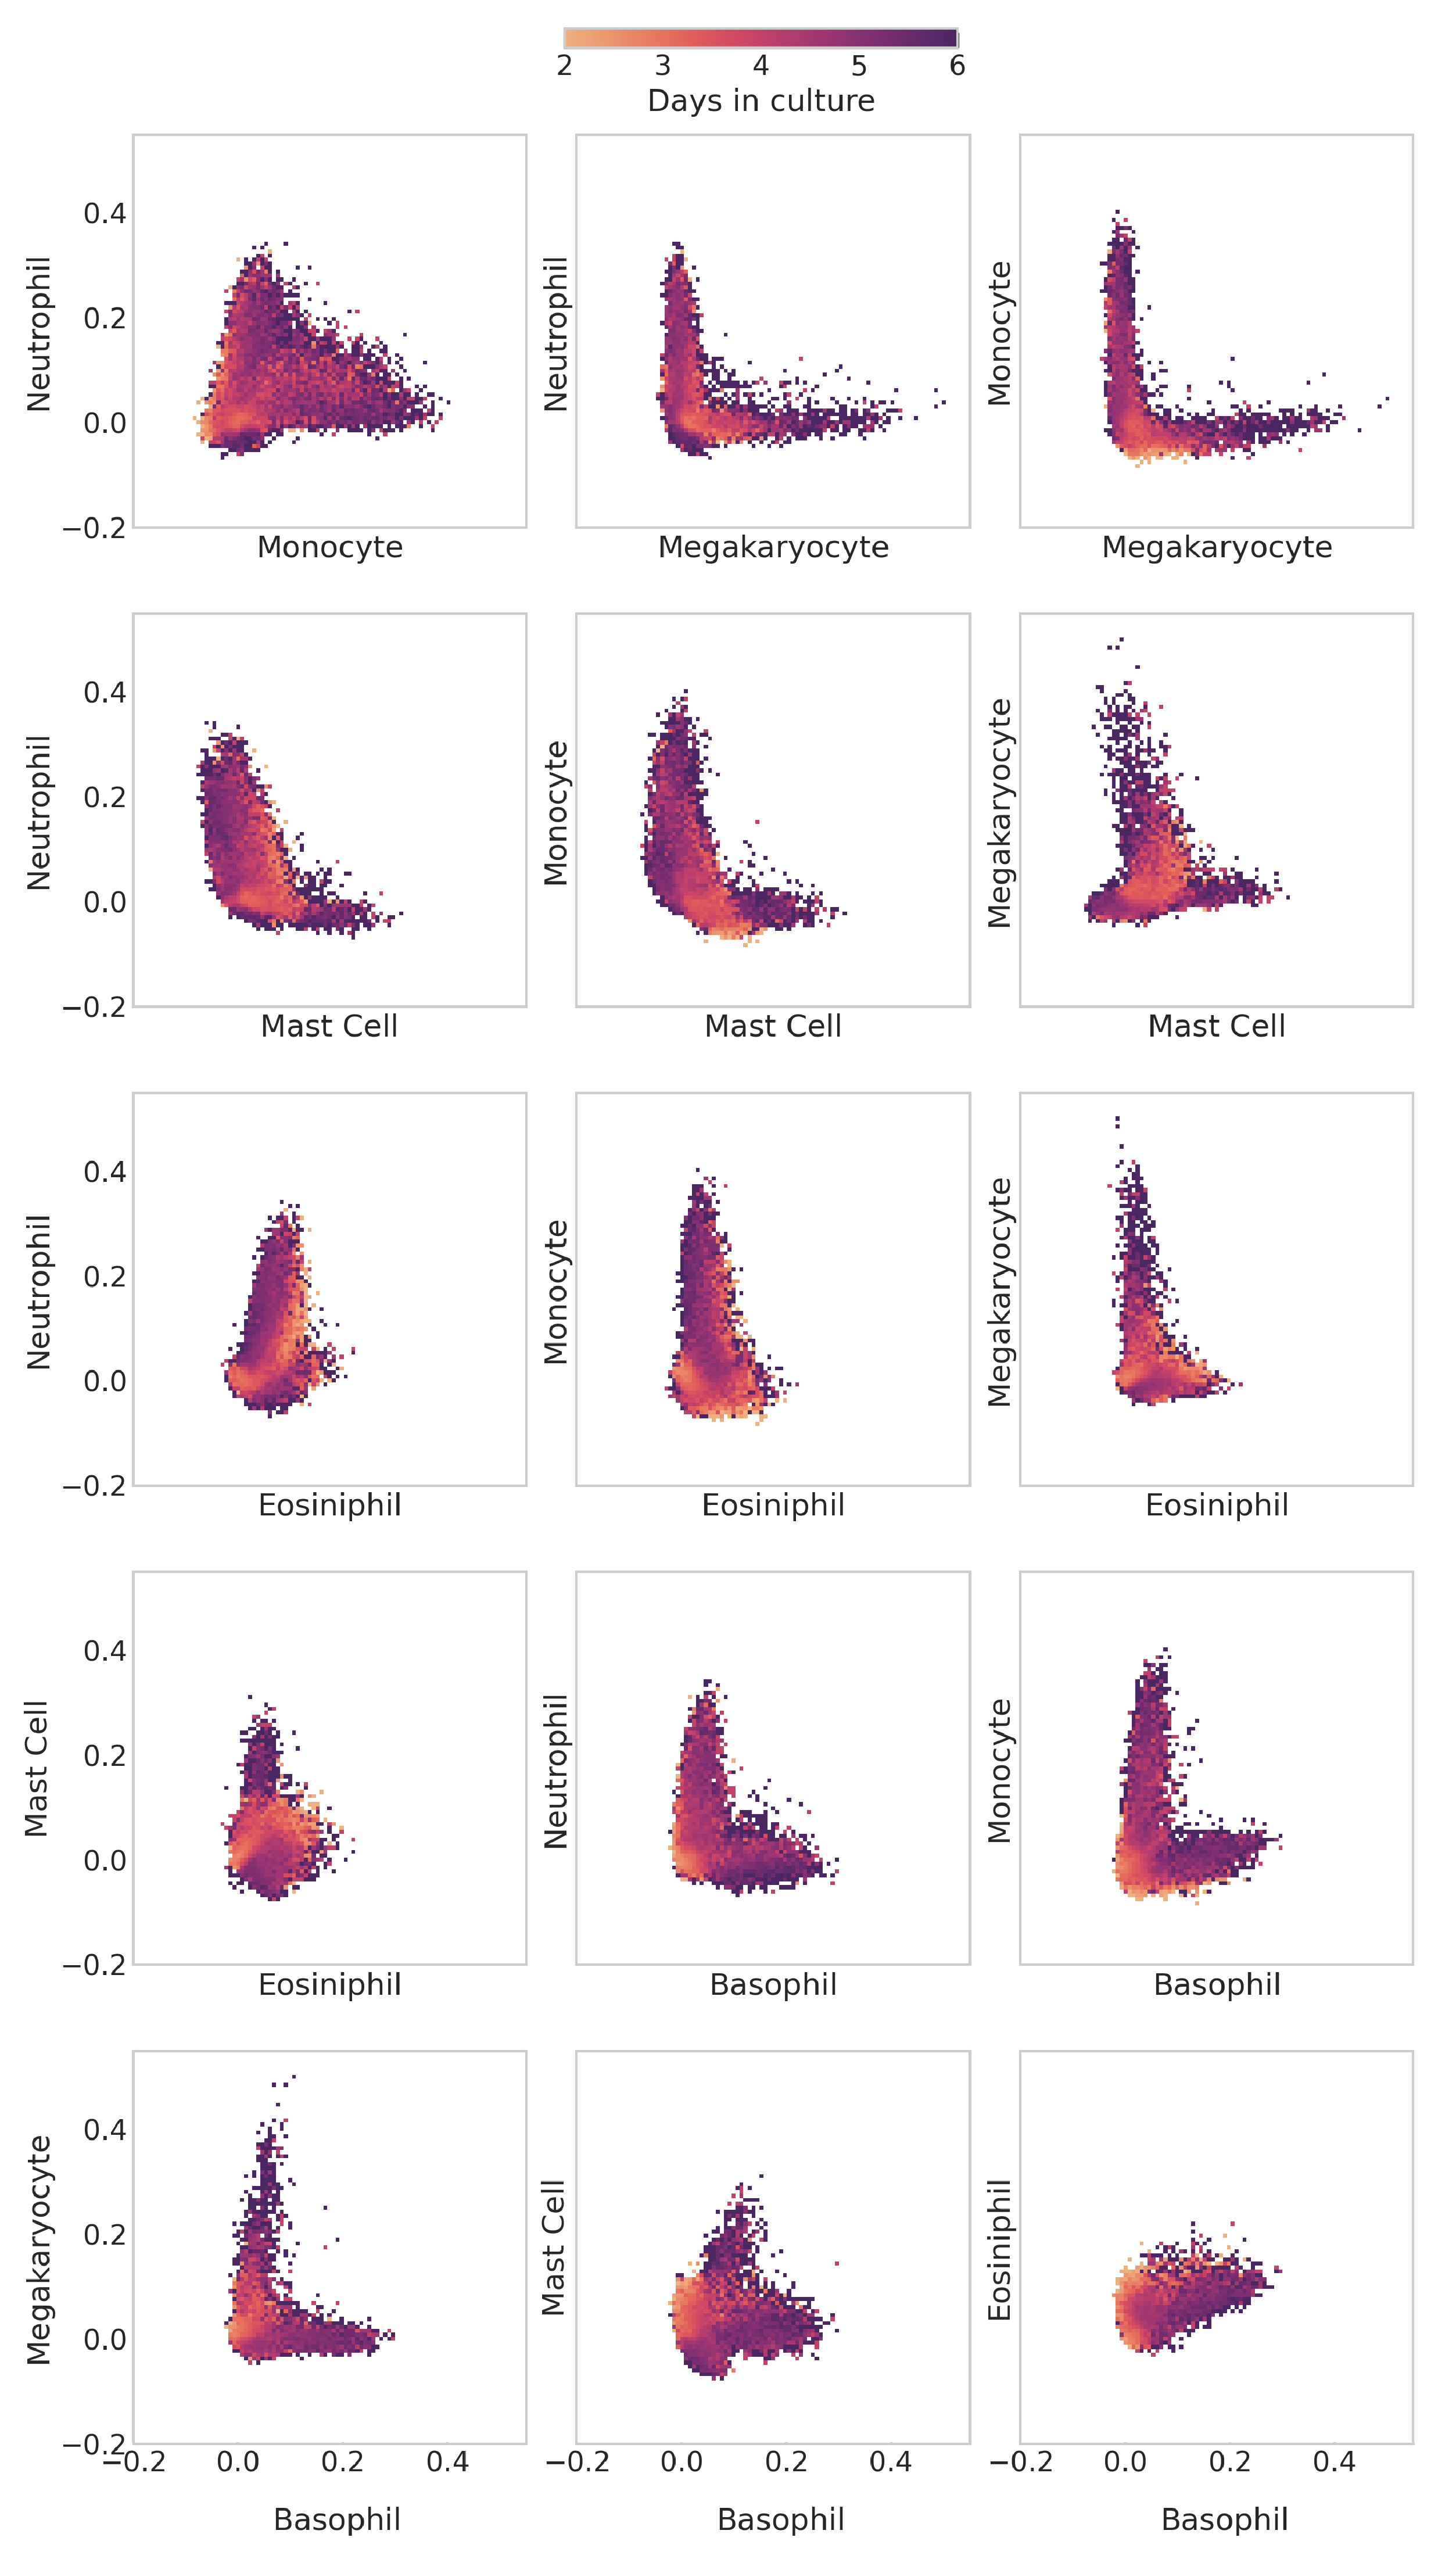
\includegraphics[scale=0.59]{figs/hem mature hists.png}
	\caption{Comparing differentiation of hematopoietic cells between mature types. As in figure \ref{hem progenitor}, the plots shown here are 2D histograms of all of the in vitro clone families from Weinreb et al. The x-axis and y-axis of each histogram indicate the scTOP score of the labelled mature type. Each bin of the histogram is colored by the average day in culture of the data points that fall within the bin.  Some pairs of types have cells with high scores of both types. This is apparent in the neutrophil-monocyte histogram, which presents a continuous spectrum of scores from the horizontal axis to the vertical. Other pairs of types only have cells expressing one type or the other, as in the L-shaped neutrophil-megakaryocyte histogram.}
	\label{hem mature}
\end{figure}


\section{Discussion}
{\color{red}: We will revisit after finalizing above... here is just some preliminary comments}

scTOP successfully quantifies cell transitions and enables direct comparison between datasets at the level of individual cells. Using a wide range of data from various sources and species, we have shown that scTOP scores identify cell type in agreement with existing annotations without being limited to discrete cluster labels. scTOP scores provide clear and meaningful axes to visualize differentiation, as shown in the cases of epithelial lung development and hematopoietic specification. The input assumptions of our algorithm are explicitly defined by the reference basis, and the results are deterministically determined by linear algebra; scTOP does not require parameter tuning or stochastic machine learning. {\color{red}: PM should add it is fast}

By assigning a continuous value to cell identity, scTOP opens the door to numerical analysis of cell fate decisions. By tracking cell type, it is possible to obtain detailed information on which transitions are possible in vivo. This will provide evidence for mapping out cell lineage trees leading from progenitors to fully-specified fates. By plotting the scTOP scores of differentiating cells, it is possible to see which cell types are mutually repressive and which are close relatives in the lineage tree. Emerging technologies like Live-seq [citation] promise to allow scRNA-seq of live cells without destroying them, and combining this capability with scTOP would allow scientists to track the process of specialization in individual cells without having to settle for lineage tracing of clones.

In addition to revealing in-vivo developmental pathways, scTOP can measure fidelity of engineered cells, as demonstrated in Herriges et al. By locating a cell in cell type space, it is possible to compare the results of directed differentiation protocols and determine which protocol provides the desired result. scTOP can guide reprogramming on a granular level in addition to probing which transitions are possible.

By projecting from gene expression space to cell type space, we can directly track cells in the cell decision landscape. As discussed in Saez et al.\cite{saez_dynamical_nodate}, such an embedding is a crucial step in verifying theoretical models of cell decisions. Many landscape geometries and dynamical systems have been proposed to explain how cell type is decided, but experimental evidence is necessary to test the validity of theoretical models. By providing coordinates in the cell decision landscape, scTOP bridges the gap between theory and experiment.

\section*{Acknowledgments}
We acknowledge useful discussions with Jason Rocks and Robert Marsland. The work was funded by a grant to the Boston University Kilachand Multicellular Design Program (to DK and PM) and NIH NIGMS 1R35GM119461 to PM. We also acknowledge programming support from Alena Yampolskaya.


\section*{Appendix}
\beginsupplement
\subsection{Pre-processing} \label{preprocessing}
The raw scRNA-seq count data for each dataset was downloaded as a matrix of genes and cells. An example of such a matrix is shown in step 0 of figure \ref{FIG:supp1}, where each row is a different gene and each column is a different cell. Throughout this figure, the histogram to the right of each step shows the distribution of entry values for the first column (cell) in the matrix, and the histogram below the step shows the distribution of entry values for the second row (gene Rpl7) of the matrix. The histograms are presented as examples of how the distributions (for each cell and for each gene) of gene expressions change as the data is preprocessed.

In the first step of preprocessing, each cell is normalized independently. This step is taken because we generally assume that every cell will have approximately the same amount of mRNA at any given moment. In other words, we expect the sum gene expression levels to be roughly the same across all cells. This step adjusts for differences in sum gene expression that may be caused by technical errors in the RNA sequencing process, such as some genes being amplified more than others and resulting in a cell appearing to have far more RNA. 

We want scTOP to be able to compare cells across sequencing conditions, so we want to transform the normalized RNA counts into quantities that are centered around the mean expression level. Z-scores are exactly such a quantity; they measure the number of standard deviations away from the mean. To calculate the z-scores after step 1, we convert the normalized gene expressions into percentiles by ranking each gene in a given cell from lowest to highest, then dividing by the number of genes (plus one, so that the highest-rank isn't assigned the 100th percentile). For example, if a cell has 1000 genes sampled and Rpl7 is the highest-expressing gene, it will be given rank 1000 and labeled as the 99th percentile. If two or more genes are tied for rank, as is the case for zero-values, they are assigned the average of the ranks they would have been assigned if they were not tied (see "rankdata" function from the Python package Scipy). To convert from percentiles to z-scores, we assumed a normal distribution with mean 0 and standard deviation 1, and applied the corresponding quantile function.

\begin{figure}
	\centering
		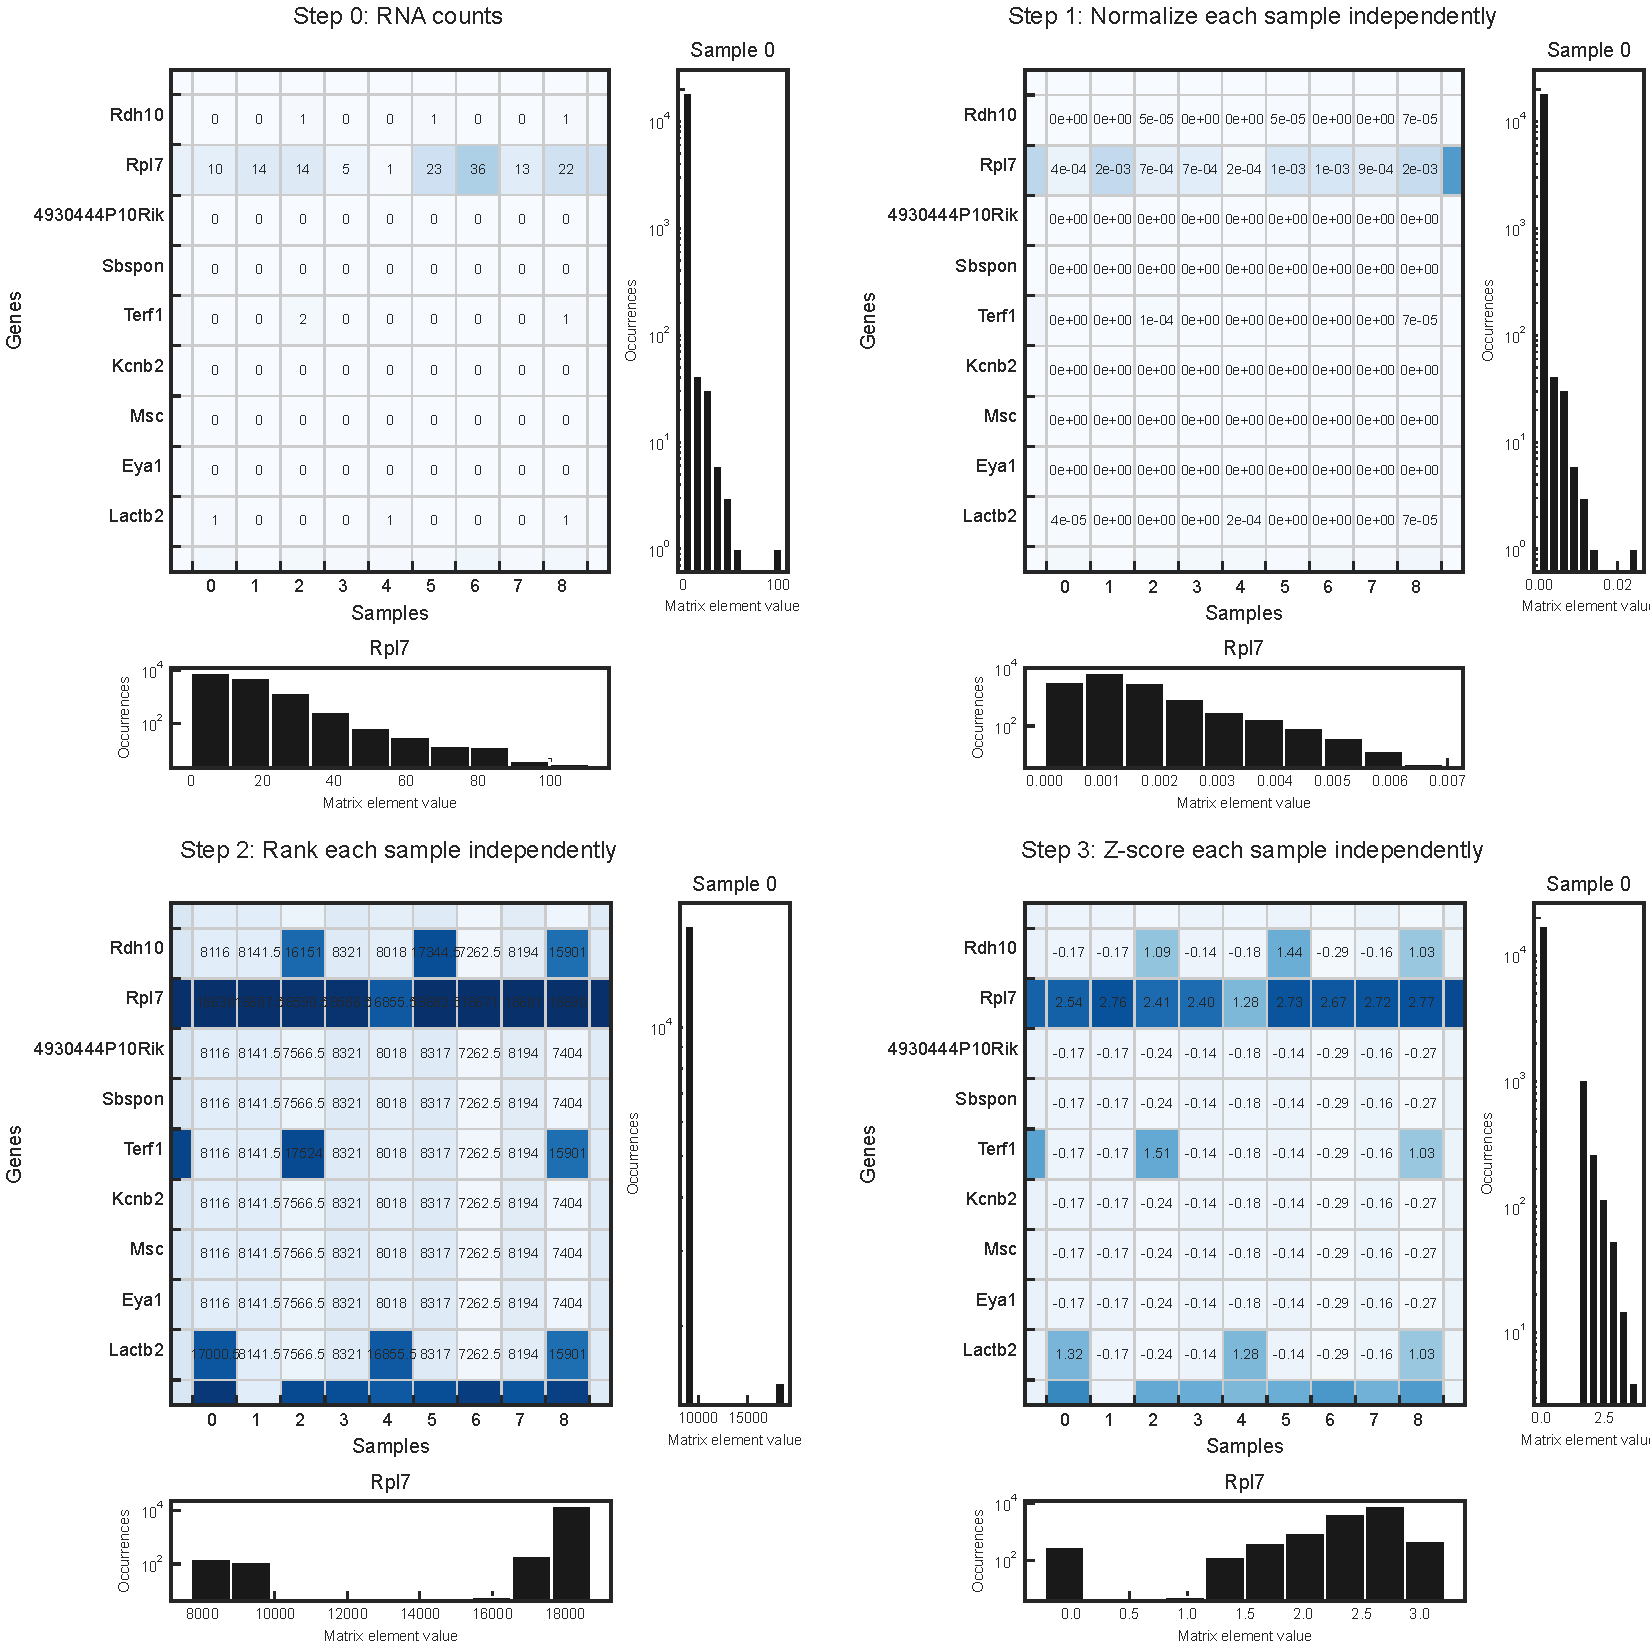
\includegraphics[scale=0.6]{figs/fig1a supplement.pdf}
	\caption{Data distributions at each preprocessing step. Step 0 shows the original RNA count matrix before preprocessing, where each entry corresponds to the number of RNA detected for a particular gene in a particular cell. The rows of each matrix correspond to genes and the columns correspond to cells. The histograms to the right of each matrix show the distribution of an example cell, while the histograms below each matrix show the distribution of an example gene. Step 1 of preprocessing is to normalize each cell. Steps 2 and 3 convert the normalized gene expressions to z-scores. Step 2 ranks the genes in each cell according to magnitude and converts the rank into a percentile. Step 3 uses a quantile function, assuming a normal distribution with mean zero and standard deviation one, to convert from percentiles to z-scores.}
	\label{FIG:supp1}
\end{figure}

\subsection{Reference basis construction}\label{basis construction}
Creating an appropriate reference basis is vital to the accuracy of scTOP. There are many existing scRNA-seq atlases, such as the Mouse Cell Atlas; using them with scTOP requires some amount of curation. For each reference dataset, we took an average over each population corresponding to a given cell type. The average gene expression profiles were preprocessed, and then became the reference profiles for each cell type. Certain cell types from each atlas were dropped for various reasons, such as not including enough cells, being poorly defined (e.g. not enough marker genes to distinguish that cell type from others), etc.

Ensuring that each reference gene expression profile sampled enough cells was essential. This is because the number of cells determines how well-sampled the reference cell type is. Although cell types have distinct transcriptomic patterns, they are not all transcriptomically identical. There are variations in gene expression levels between cells of the same type due to differences in cell-level processes such as cell division or environmental stimuli. Averaging over a population of cells which are some cell type X creates an approximate gene expression profile of the archetypal X cell. 

\subsubsection{Mouse Cell Atlas}
The Mouse Cell Atlas (MCA) contains hundreds of thousands of cells from tissues across the mouse body at various stages of development. For the reference basis created from the Mouse Cell Atlas (MCA), we dropped cell types that had fewer than 100 cells. For cell types that had greater than or equal to 100 cells, we averaged across the entire population for each one, then preprocessed. For cell types that were divided according to high expressions of various genes, we combined them into one cell type. For example, the original MCA contained dozens of clusters of mammary gland secretory alveoli cells such as "secretory alveoli cell, Hes1 high" or "secretory alveoli cell, Gpx3 high." These were all combined into one cell type, "mammary gland secretory alveoli." This is because we wanted each reference basis type to act as an archetype rather than a perfect representation of every possible iteration of a cell type; each reference type represents a basin of attraction, and the basins were defined by the overall cell type, not whether individual genes were particularly high within that cell type. We cleaned each of the MCA type labels and ended up with cell types defined by the organ of origin, specific cell type, and time point of collection (e.g. "lung ciliated cell week 6-10"). The time points of cell types in the MCA were either E14.5 or somewhere between week 6 and week 10 post-birth.   The resulting reference basis contained 221 cell types.

\subsubsection{Hematopoietic reference data}
For the hematopoietic dataset, we excluded erythrocytes because the authors used only one marker gene was used to annotate cells of that type. This resulted in many cells having a high erythrocyte score because selecting cells according to the expression of one gene does not sufficiently define the red blood cell population.

{\color{red} MY: Discuss the rest of the reference bases} 

\subsection{Accuracy measures}
For table \ref{table:1}, the top1 accuracy was determined by applying scTOP to a cell, finding the type with the highest score, and checking whether that type matched the cell's "true type." Top3 was similarly determined, except instead of just checking the highest-scoring type, we checked whether the true type was included in the top 3 highest-scoring types.

By looking at the scTOP scores for cells whose true type did not match the reference type, we set a score of 0.1 as the lower bound for identifying a type. As shown in figure \ref{robustness hists} (c) and (f), when the reference type does not match the sample type the scores for individual cells fall well within [-0.1, 0.1], even when most of the reference basis is missing.

In table \ref{table:1}, we labeled cells as "unspecified" if the highest scTOP score was less than 0.1. This provides a useful metric for determining whether a query cell belongs to one of the cell types in the reference basis. If the highest scTOP score is lower than 0.1 for a query cell, this indicates that the reference basis lacks the relevant types or was poorly constructed (see appendix \ref{failure_cases} for a discussion of ill-defined bases). 

scTOP can only identify cells that exist within the reference basis. As such, the accuracy scores were calculated only for the cells whose true type (as determined by the annotations from the authors) was included in the reference basis for the corresponding analysis. For cells whose true types were not represented in the basis, the unspecified rate was very high. This indicates that the rate of false positives is very low.

\subsection{Robustness of scTOP}
scTOP is consistent between iterations of the algorithm, and it is robust to changes in the reference basis. As shown in figure \ref{robustness hists}, many scTOP scores do not change significantly even when most of the reference basis is removed. Generally, scores for cells that match the reference type do not change much even when only 25\% of the original basis is retained (figure \ref{robustness hists} (d), (e)). The largest difference occurs for cells that are similar to the reference type, such as the AT1 score for AT2 cells (figure \ref{robustness hists} (g)). These scores tend to increase, because removing other types from the basis reduces the ability to de-correlate effectively. In other words, scTOP is more likely to confuse similar types when it has fewer reference types to compare. This effect is most apparent when relevant types are removed from the basis. Figures \ref{robustness hists} (j) and (k) show that all lung types score higher for AT1 and AT2 when only lung alveolar types are included in the basis. Figures \ref{robustness hists} (c) and (f) show that irrelevant scores, such as bladder and thymus cells, do not change much even when large portions of the basis are removed. scTOP does not confuse sample cells for types that are dissimilar even with a small reference basis because there is no need to de-correlate between types that are naturally not correlated.

\subsubsection{Cases where it doesn't work}\label{failure_cases}
The performance of scTOP relies on the quality of the reference basis. scTOP is expected to give inaccurate results in cases where the reference basis is ill-defined. The underlying assumption of the algorithm is that the reference basis consists of accurate gene expression profiles of cell types that are attractor basins. In other words, the reference types are assumed to represent stable cell types rather than cell states that are on the path to the true cell type basins. For example, scTOP performs poorly when using a reference basis made up of embryonic types that are too early in development, because the cell types are not differentiated from one another. Early embryonic cells are not specified yet, so they are not reliable references for cell type.

The reference cell types should refer to attractor basins. The other part of the assumption is that the reference types should be accurate profiles of those attractor basins. As discussed in appendix \ref{basis construction}, reference types are created from averaging over cells, and the more cells included in this average the better-sampled the type is. As expected, scTOP gives unreliable results when the reference gene expression levels don't accurately reflect the true cell types' gene expression levels. An important factor in the accuracy of scRNA-seq is the amplification step: after RNA is extracted, it is amplified to improve the sensitivity of sequencing, but not all RNA is amplified at the same rate. This results in inflated counts for some genes but not others. Unique molecular identifiers (UMIs) are vital for reducing the inflating effect of amplification [CITE umi paper]. UMIs tag the RNA before amplification, and are present post-amplification; this makes it possible to see which amplified RNA came from the same original molecule, and prevents uneven double-counting of RNA. We have found that scTOP gives more accurate results when used with reference and query datasets that use UMIs, compared to scTOP results using data that did not use UMIs.

\begin{figure}
	\centering
		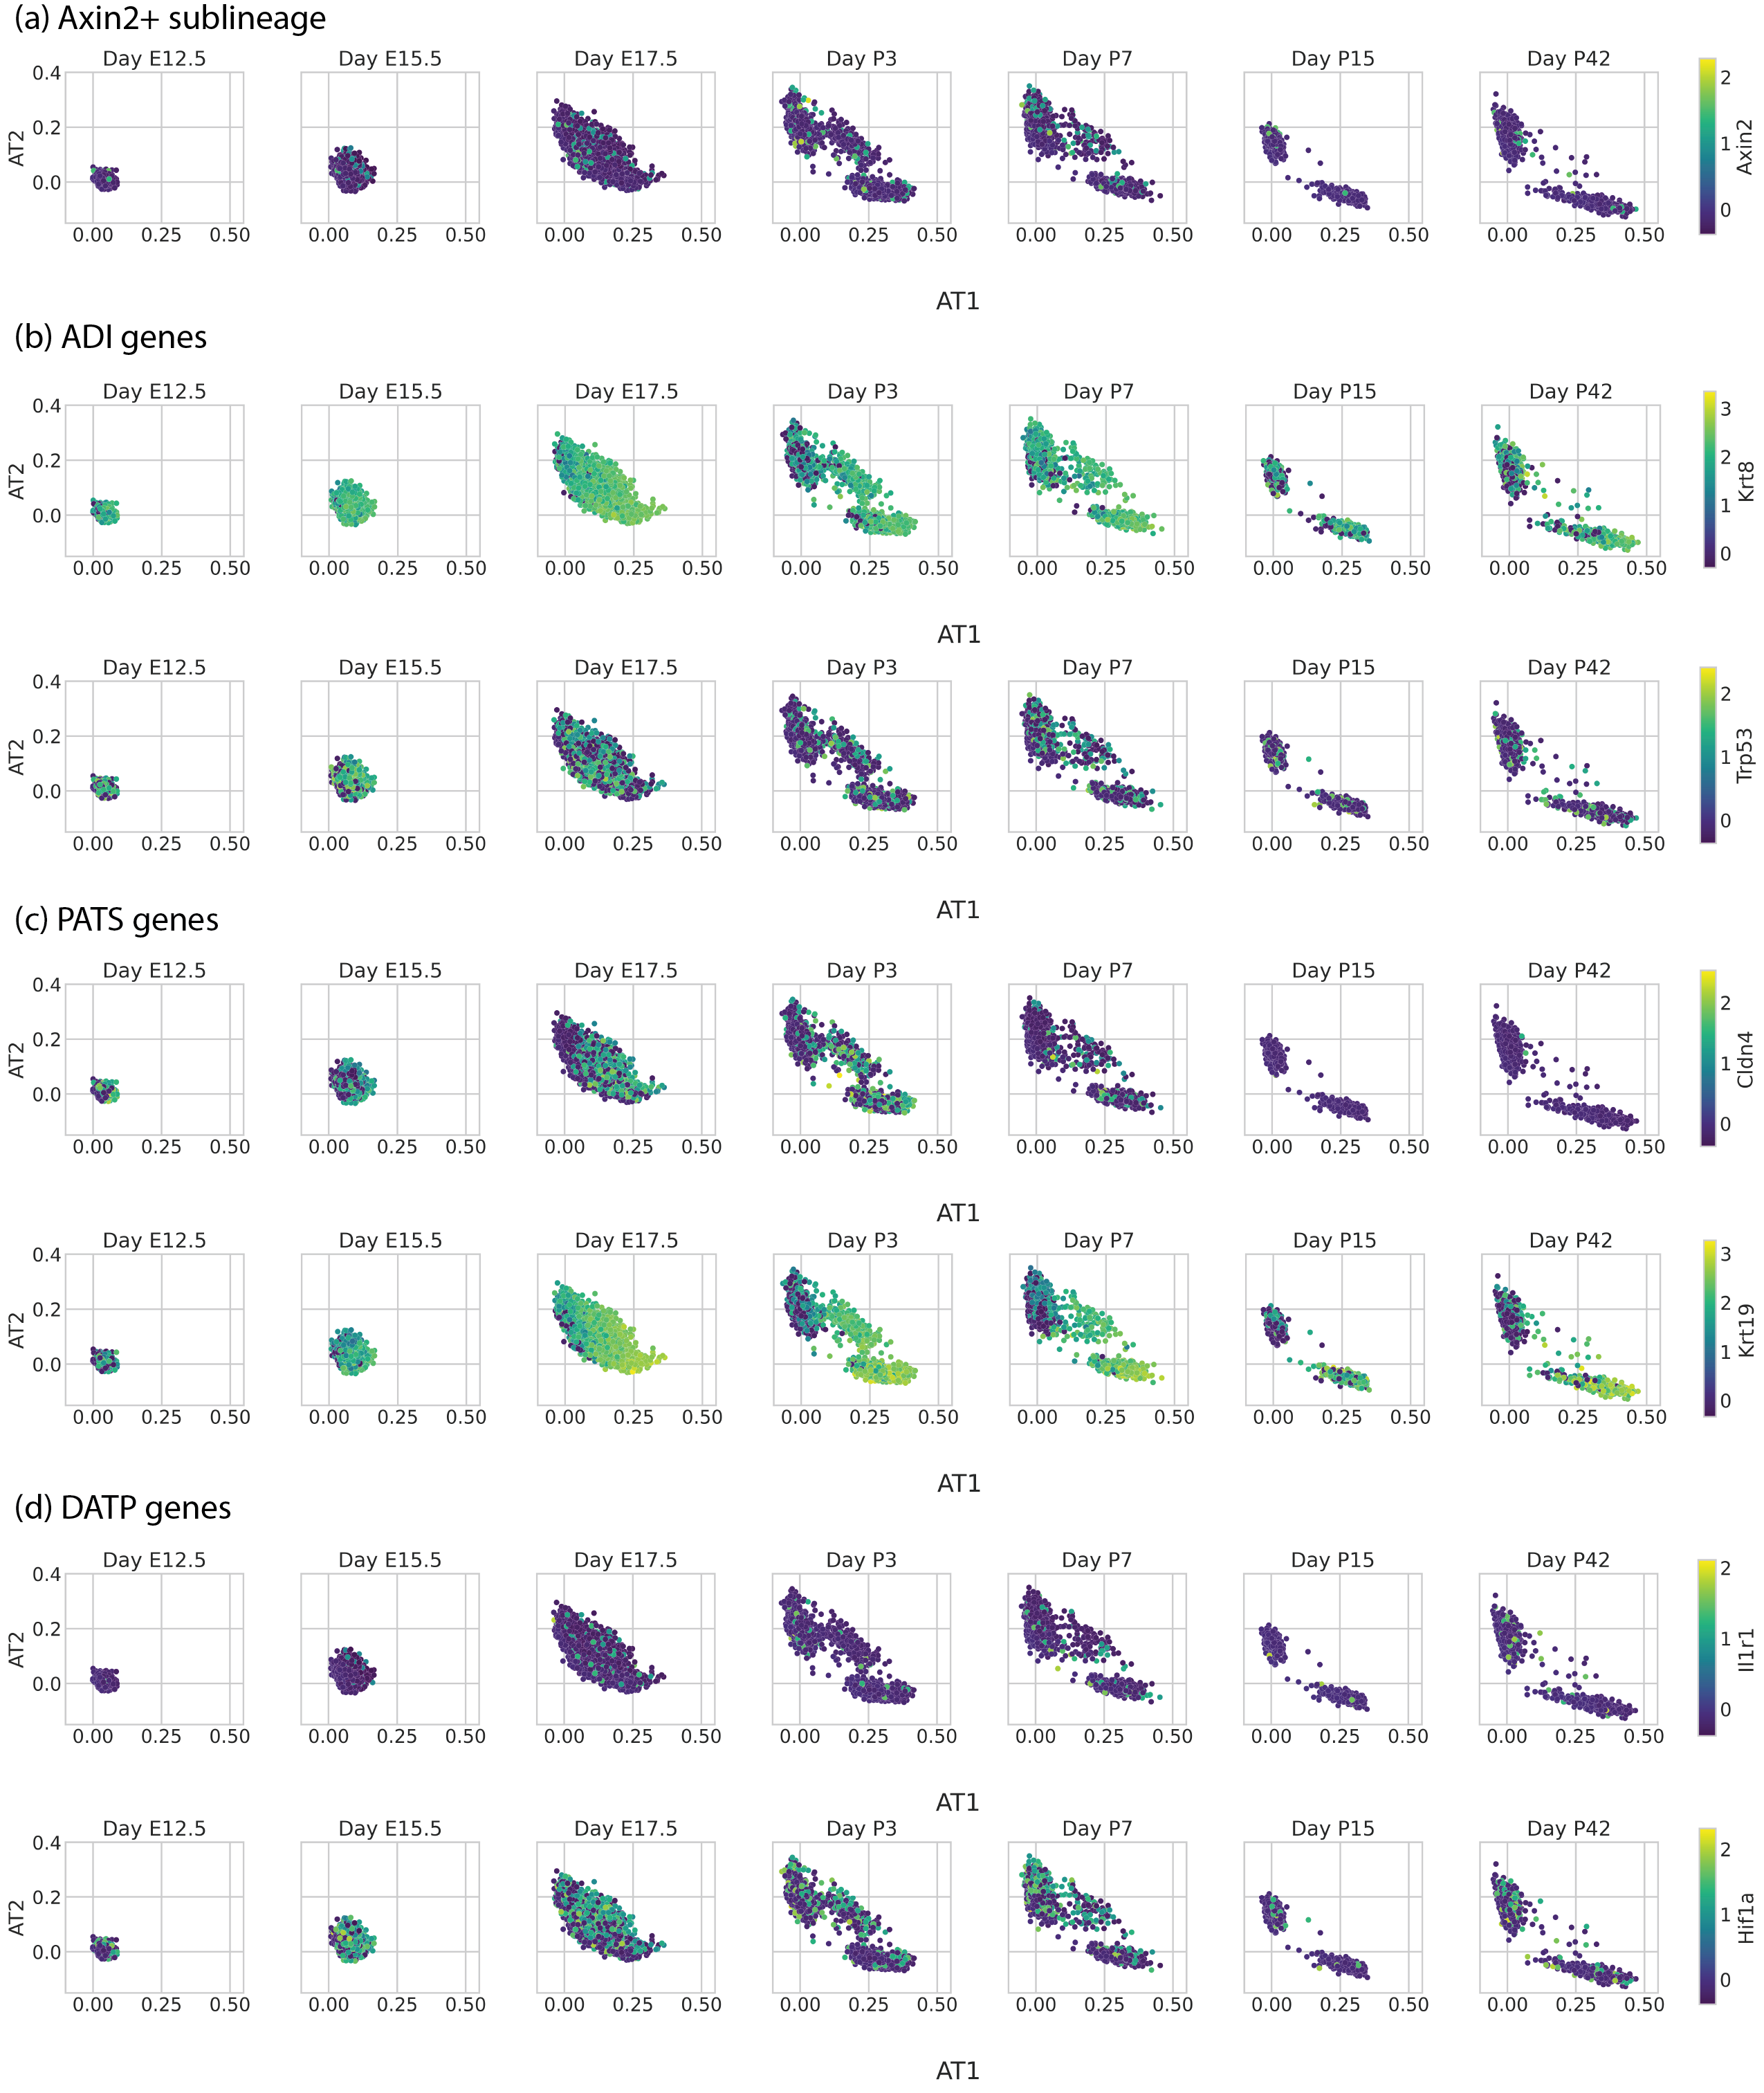
\includegraphics[scale=0.8]{figs/LungMAP genes.png}
	\caption{The AT1/AT2 combination state (most apparent in days P3 and P7) do not uniquely express genes of AT1/AT2 transitional states described by previous papers. Alveolar cells from Zepp et al. are plotted on AT1 and AT2 axes, separated by day. Each cell is colored by the expression z-score of a particular gene, and the particular gene is different in each row. The gene used to color the cells is indicated by the color bar on the far right of each row. (a) Alveolar cells colored by Axin2+, showing that the AT1/AT2 combination cells do not appear to belong to the Axin2+ sublineage described by [CITE]. (b) Alveolar cells colored by Krt8 and Trp53 expression, which are genes corresponding to alveolar differentiation intermediate cells (ADI) described by [CITE]. AT1, AT2, and the combination AT1/AT2 state all express Krt8 and Trp53 at similar levels. (c) Alveolar cells colored by expression of pre-alveolar type-1 transitional cell state (PATS) genes [CITE]. AT1, AT2 and the combination AT1/AT2 state all express Cldn4 at similar levels. AT1 and AT1/AT2 combination cells both express Krt19 at similar levels, although AT1 cells express the gene at higher levels. (d) Alveolar cells colored by expression of damage-associated transient progenitor (DATP) genes [CITE]. AT1, AT2, and the combination AT1/AT2 state all express Il1r1 and HIF1a at similar levels. }
	\label{LungMAP genes}
\end{figure}

\begin{figure}
	\centering
		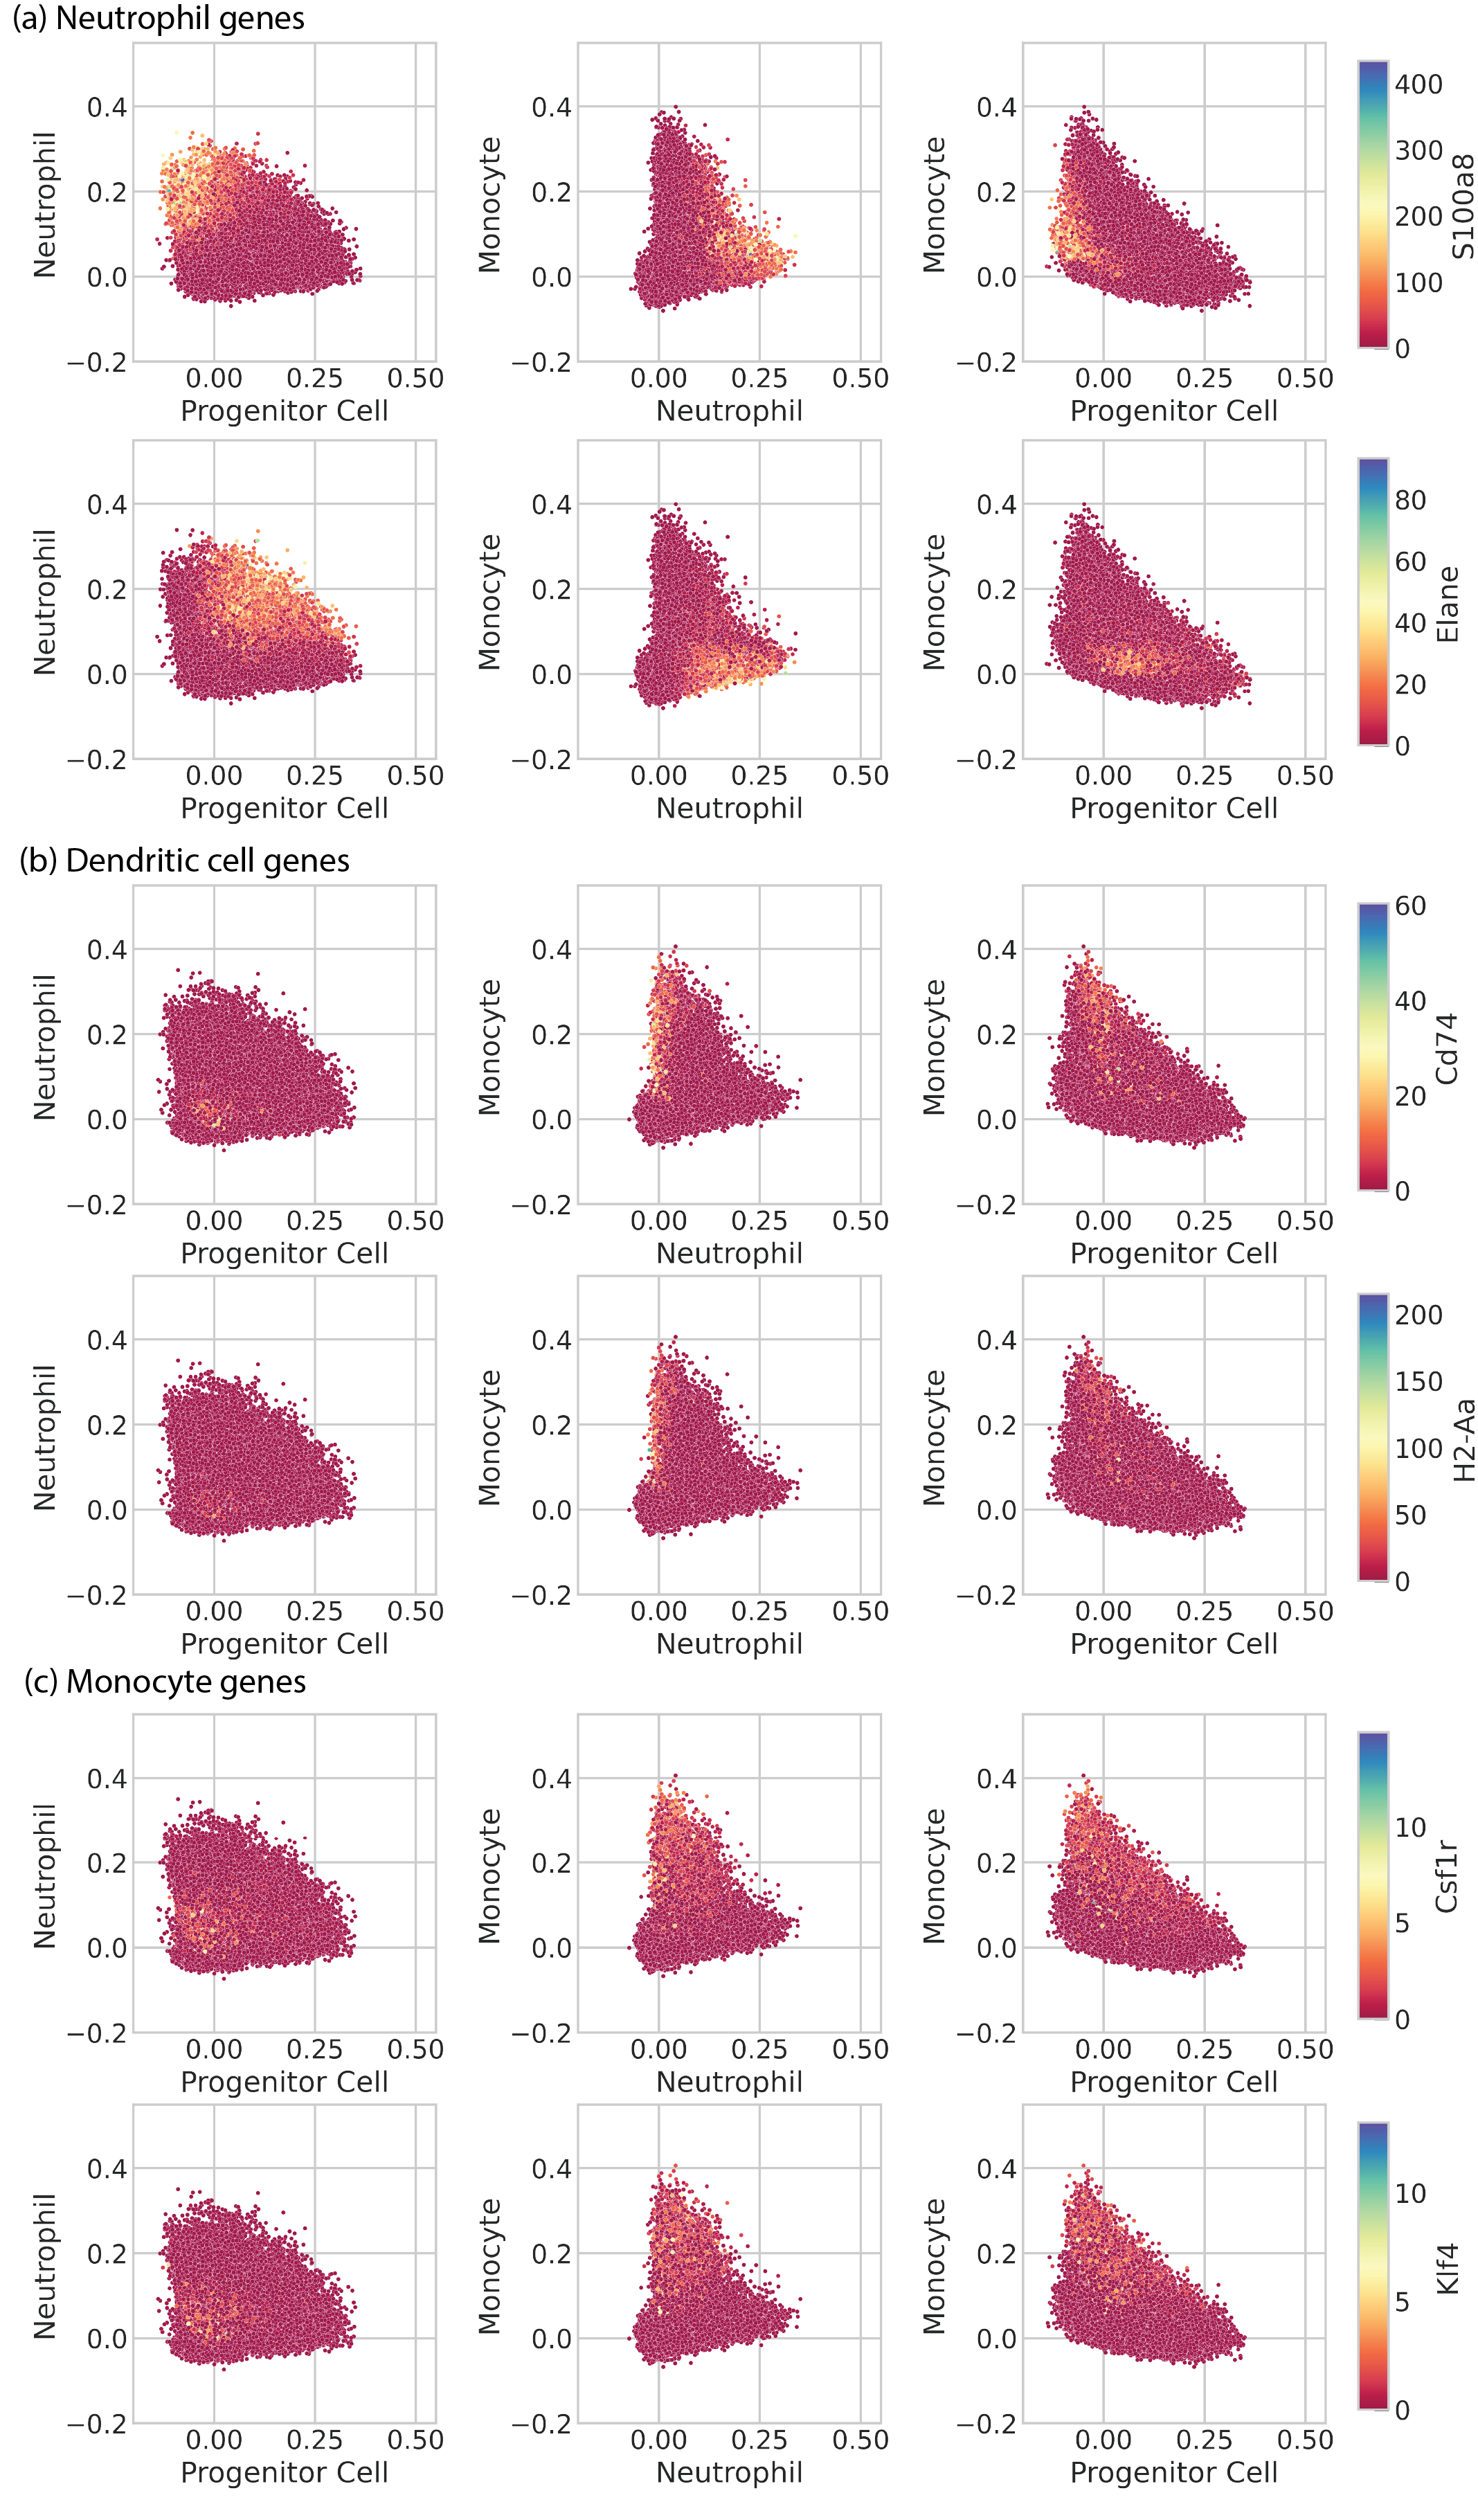
\includegraphics[scale=0.72]{figs/hem genes.png}
	\caption{Scatter plots of in vitro hematopoietic clone families from Weinreb et al., with scTOP scores for progenitor, neutrophil, and monocyte types, and colored by normalized gene expression. In Weinreb et al. figure 4 (a), cells visualized using pseudotime inference were separated into branches. The monocyte branch appeared to have half of its cells expressing dendritic cell genes and the other half expressing neutrophil genes. This figure plots those same cells on progenitor, neutrophil, and monocyte axes, and colors according to neutrophil, dendritic cell, and monocyte marker genes. (a) Hematopoietic cells colored according to expression of neutrophil marker genes S100a8 and Elane. (b) Hematopoietic cells colored according to expression of dendritic cell marker genes Cd74 and H2-Aa. (c) Hematopoietic cells colored according to expression of monocyte marker genes Csf1r and Klf4. }
	\label{hem genes}
\end{figure}

\begin{figure}
	\centering
		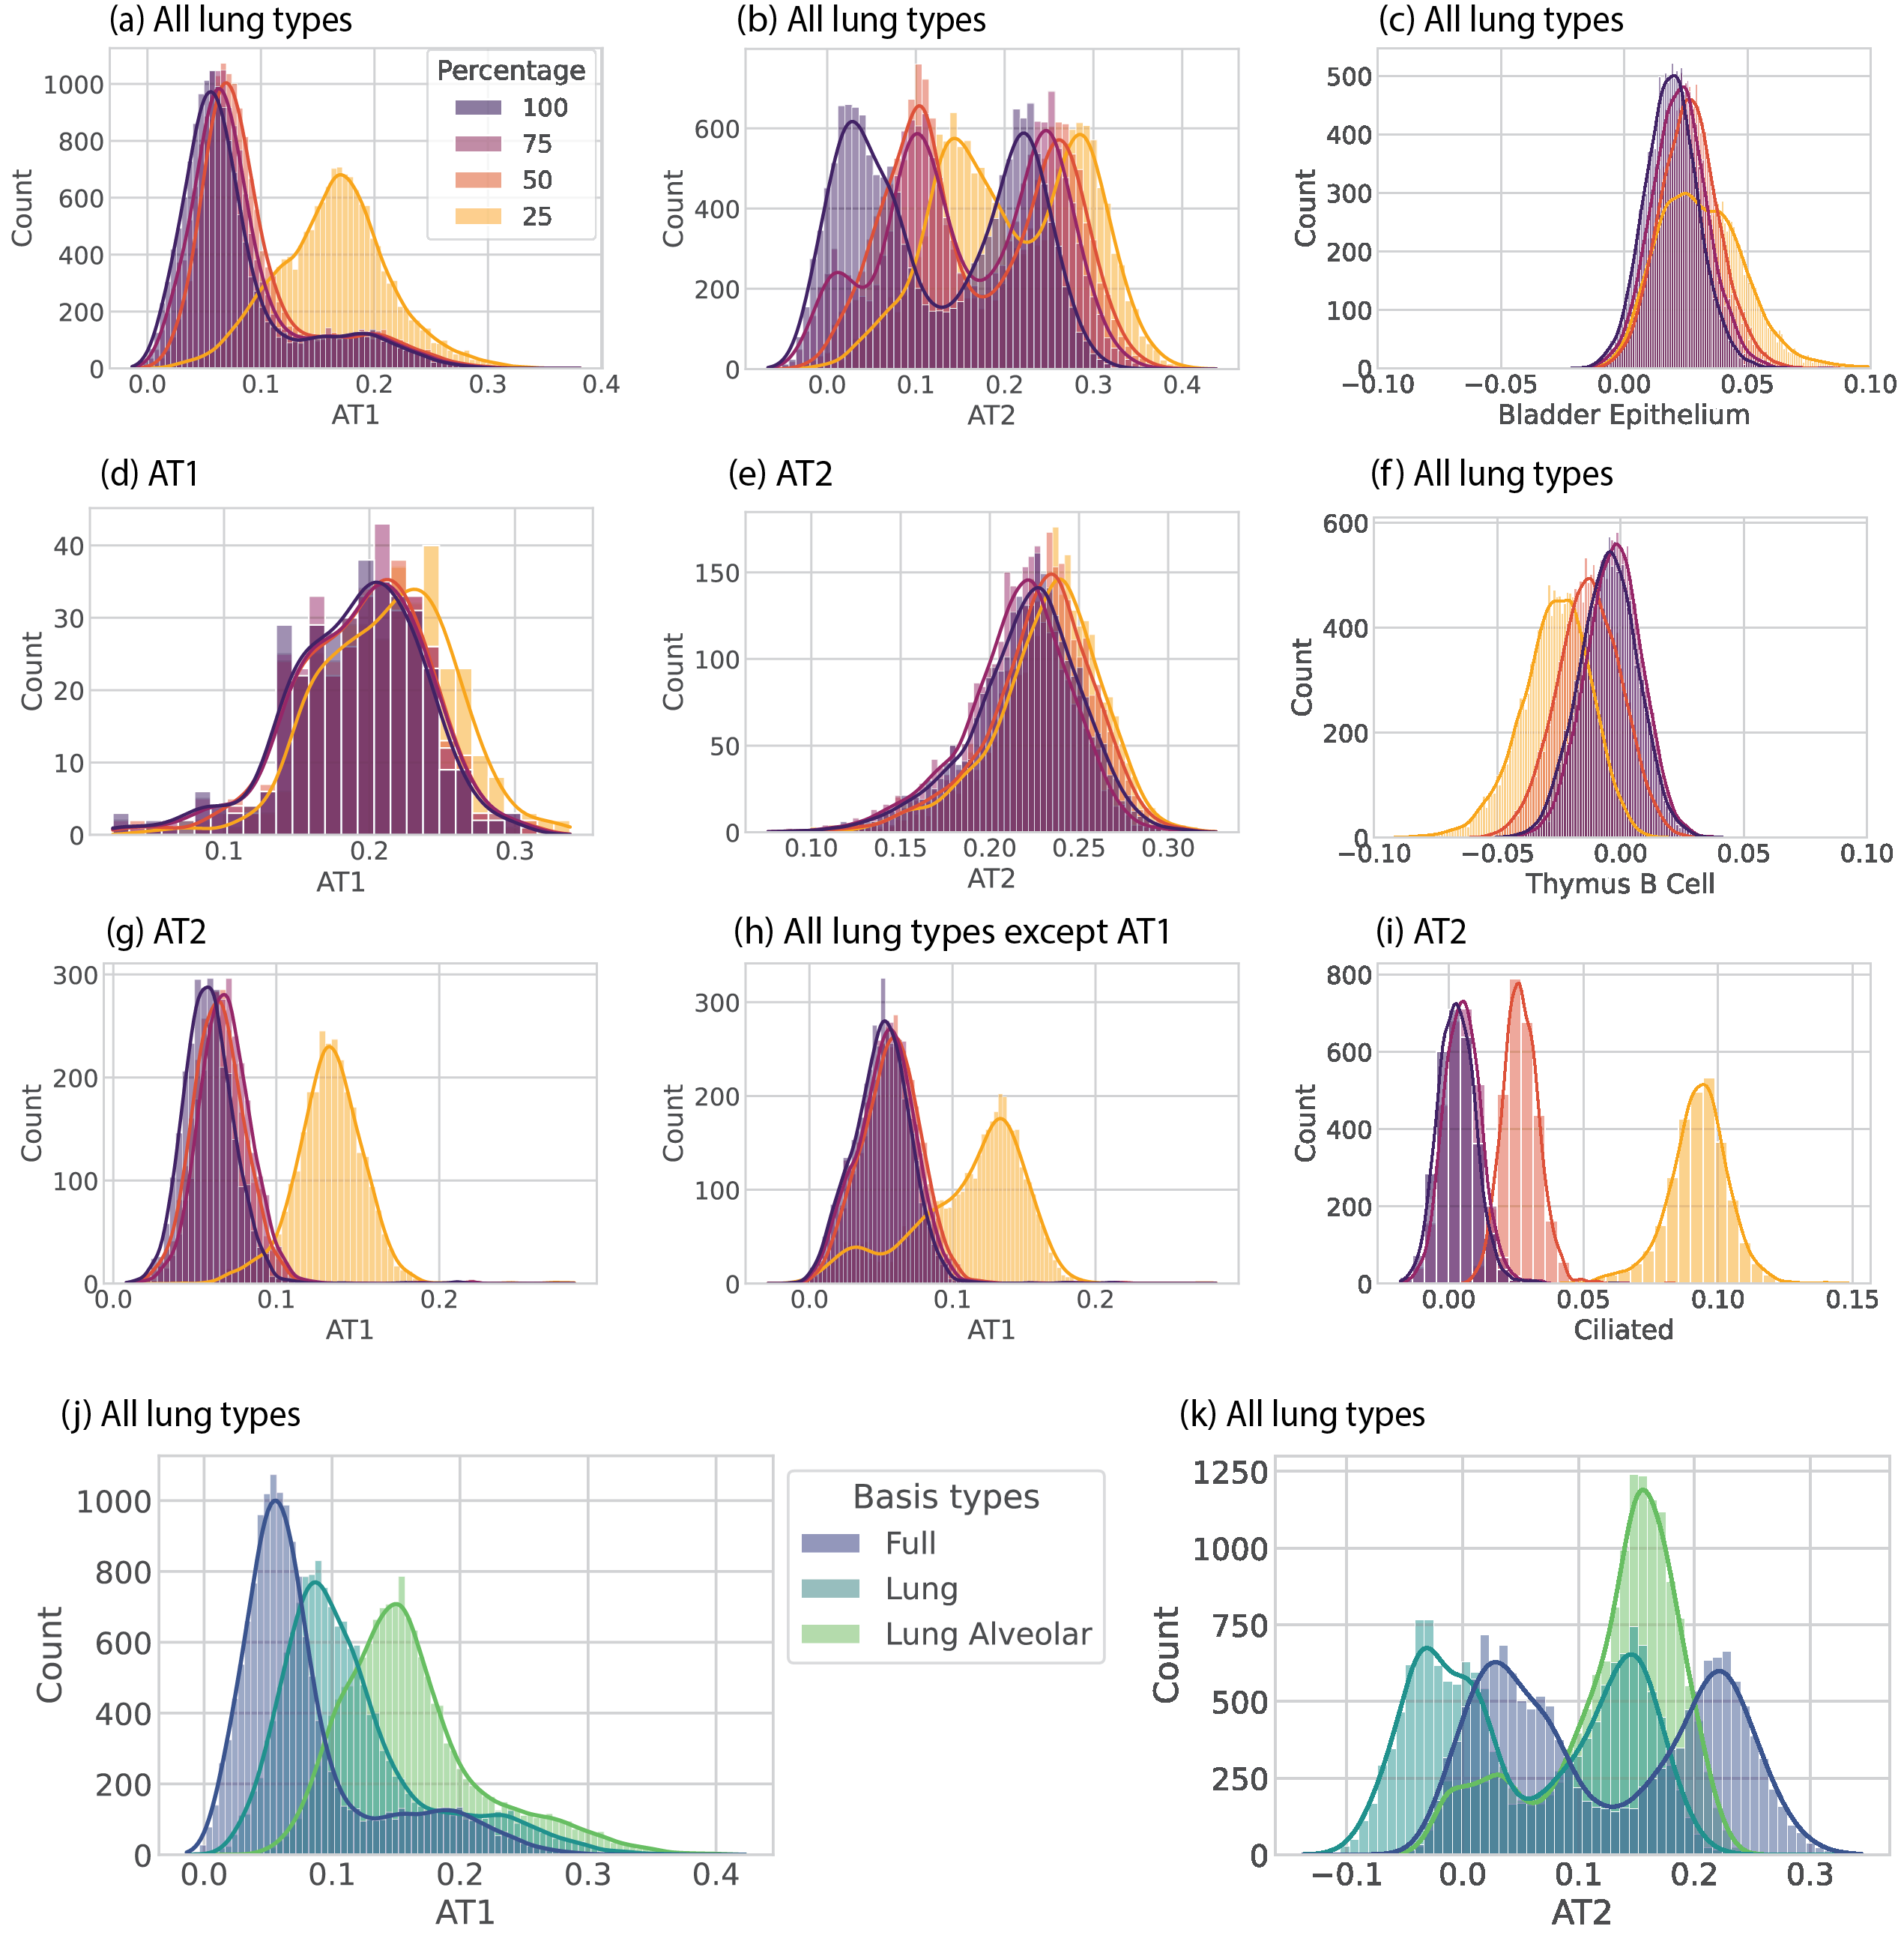
\includegraphics[scale=0.82]{figs/robustness hists.png}
	\caption{Distributions of scTOP scores for lung cells from Herriges et al., using varying portions of the Mouse Cell Atlas as the basis. the label above each plot indicates the Herriges et al. sample subset, while the x-axis label indicates the scTOP reference type. "All lung types" means that all of the lung types from the data set were included. (a) - (i) show how scTOP scores change when 25-100\% of the basis is used. (j) - (k) show how scTOP scores change when the basis is changed from the full basis (which includes many tissues and organs), to just the lung types, to just the two alveolar types. (c) and (f) show scTOP scores for random irrelevant types, Bladder Epithelium and Thymus B Cell, to show that the scTOP scores remain low for types that don't match the sample.}
	\label{robustness hists}
\end{figure}

\bibliography{export-data.bib}

\end{document}